
\documentclass[12pt,a4paper]{article}

\usepackage[english]{babel} 
\usepackage{amssymb}
\usepackage{amsmath}
\usepackage{txfonts}
\usepackage{mathdots}
\usepackage[classicReIm]{kpfonts}
\usepackage[margin=1in]{geometry}
\usepackage{graphicx}
\graphicspath{{images/}}
 

\newcommand{\nand}{\, \wedge \,}
\newcommand{\nexist}{\,\, \exists \,\,}
\newcommand{\ind}{\indent\indent}
\begin{document}

\begin{flushleft}

\includegraphics[scale=0.8]{inha_logo.eps}  
\end{flushleft}

\begin{flushright}


	\bigskip
	\large{Database Application and Design (SOC-3060) -- Spring 2019}\\
	\bigskip\bigskip
	\Huge\textbf{Database System Report} \\
	\bigskip\bigskip
	\Large \textbf{for} \\
	\bigskip\bigskip
	\Huge \textbf{The Uzbek Tragedy} 
	\bigskip\bigskip\bigskip
	
	\large Prepared by Anvarjon Yusupov (u1610026)\\
			Jamoliddinkhuja Odilkhujaev (U1610092)\\
			\underline{Mokhlaroyim Tuychibaeva* (U1610148)}\\ 
	\bigskip\bigskip\bigskip
	\large Davinci Union
	
	\bigskip\bigskip\bigskip
	\today
\end{flushright}

\newpage

\noindent 

\noindent 

\noindent 

\noindent 


\paragraph{1. Introduction and scope\\}
\ind \\
\ind Proposed project name is called \textbf{"The Uzbek Tragedy"} dedicated to discovering mountains in Uzbekistan with its magnificent nature, animals and plants in form of the game. The Uzbek Tragedy is a sub-type of game genre Visual Novel. \\
\ind Visual novel - is interactive game genre oriented on story-telling with the narrative style of literature and interacting with the player via sprites, choices and etc. Visual novels are often produced for video game consoles, and rarely ported to other systems\\
\ind The product will entertain users by an astonishing story with 4 main characters. Where the fate of characters will depend on the players choice. Moreover, the product will show to users Uzbek nature in its pure serenity. The animals and plants represented in the project are animals that truly inhabit in Uzbek territory. Plants and animals can be dangerous or useful, for example: if player will see wolf, definitely this is dangerous animal, while if it squirrel, animal cannot harm player, that applies to plants too, some plant can be poisonous or helpful, and it depends on players choice how to use it, because sometimes even poison can be helpful.\\
The game will attract end users with its astonishing story, the whole story takes place around 4 medical university junior students, who got into trouble, in Uzbek mountains, while they were going to have several lectures about healing herbs. The main character's name is August, he will survive after the school bus crash, so his main goal is to survive and find way home. While he travels he can find his friends and survive together or he can try to save himself and sacrifice his friends. August will have an encyclopedia, a book from his studies with various information about herbs, so if he will see unknown herb, he can reveal if it can help him or harm. Every choice of August will lead to certain consequences, so if he wants to survive, he can't be hero of justice, he has to choose who will live and who will die. \\
\ind Interface part of the project will be by Unity. Unity 3D is a cross-platform game engine and integrated development environment (IDE) for creating interactive media. It enabled the game app development for different platforms and distinct devices in a user-friendly development environment. It used to build games and the technology that executes the graphics, audio, interactions, and networking\cite{unity}. The relevance of using unity is that Unity is multi-platform and has all-in-one editor, relatively building project to any platform much easier. 

\newpage
\paragraph{2. Product perspective}
\subparagraph{2.1 Comparison\\}
\ind \\
\ind\indent The Uzbek Tragedy is one of the Visual Novel game genres, therefore there is many competitors in the world\\
\ind\indent Most popular example is Fate Stay night\cite{fate}, Katawa Shoujo\cite{shoujo}, and Everlasting Summer\cite{summer}\\
\ind\indent Here is Competitors table, which compares several similar products with the Uzbek Tragedy\\
\begin{center}
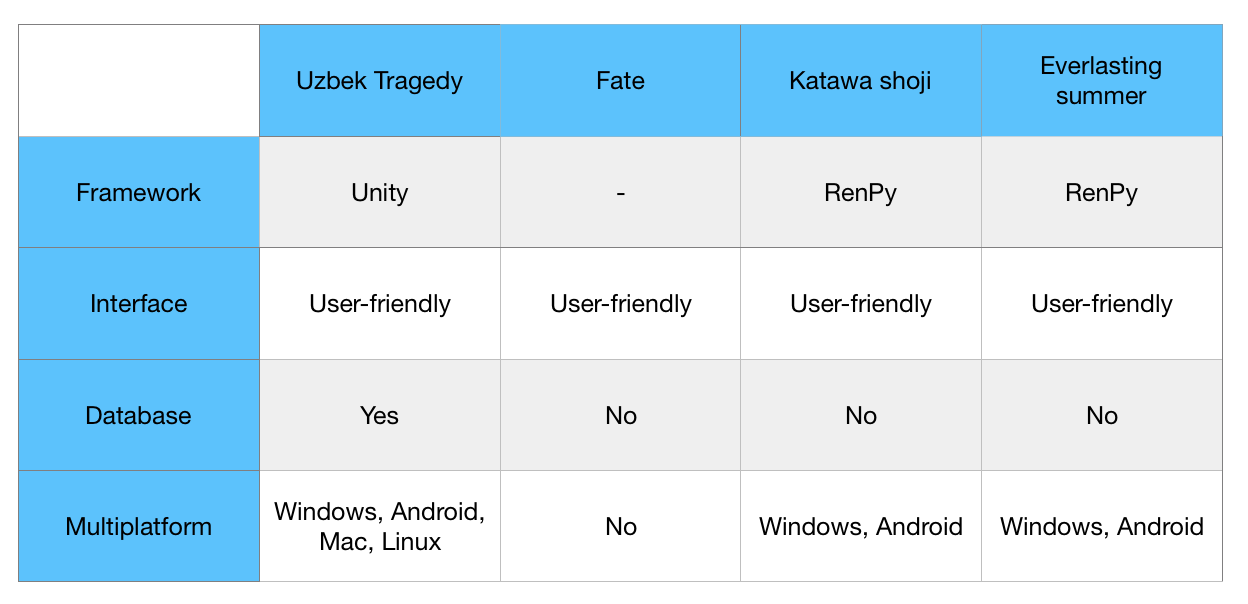
\includegraphics[scale=0.8]{images/Competitor.png} 
\end{center}
\subparagraph{2.2 Product perspective\\}
\ind \\
\ind The Uzbek tragedy is a unique product because only this project is using Database for his needs. Moreover, it is multi-platform. Because, The Uzbek Tragedy, has his own unique design, based on mountains of Uzbekistan and containing animals from Uzbekistan. 
This project uses SQLite database management system instead of MySQL for database needs because for project usage Mysql would be too heavy. SQLite self-contained, file-based database with faster speed, the game doesn't need a big amount of data, so light-weighted DBMS the best option here.\\
\ind As it is mentioned above, interface part of the project will be by Unity. Unity 3D is a cross-platform game engine and integrated development environment (IDE) for creating interactive media. It enabled the game app development for different platforms and distinct devices in a user-friendly development environment. It used to build games and the technology that executes the graphics, audio, interactions, and networking\cite{unity}. The relevance of using unity is that Unity is multi-platform and has all-in-one editor, relatively building project to any platform much easier. 
\newpage
\paragraph{3. Specific requirements\\}
\subparagraph{3.1 Logical database requirements\\}
\begin{center}

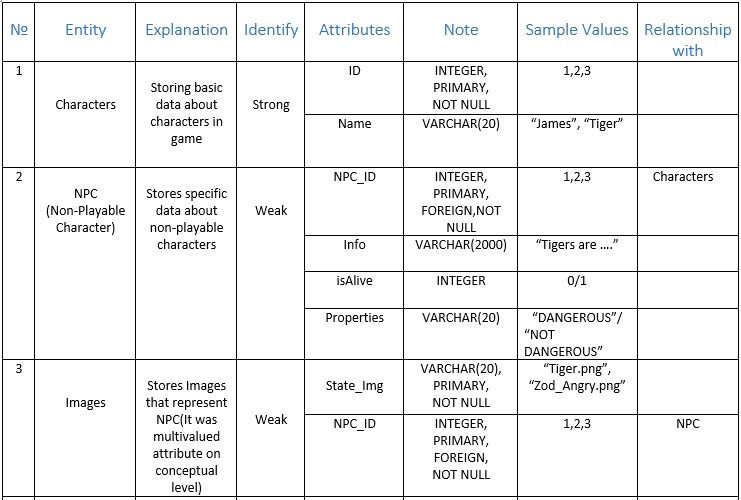
\includegraphics[scale=0.6]{images/LDR1.jpg}
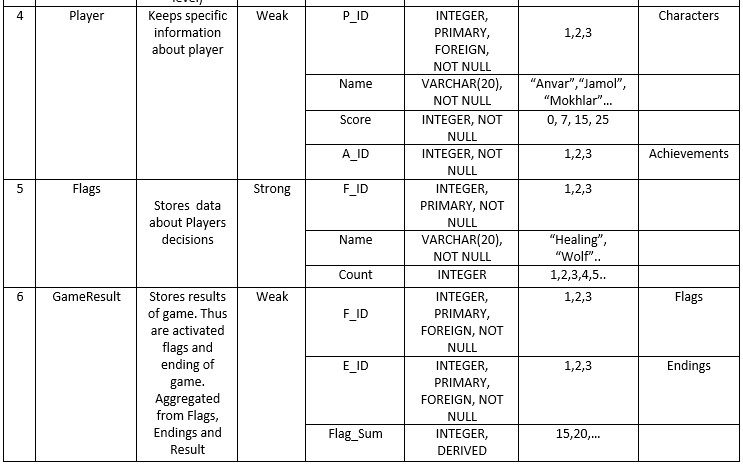
\includegraphics[scale=0.6]{images/LDR2.jpg} 
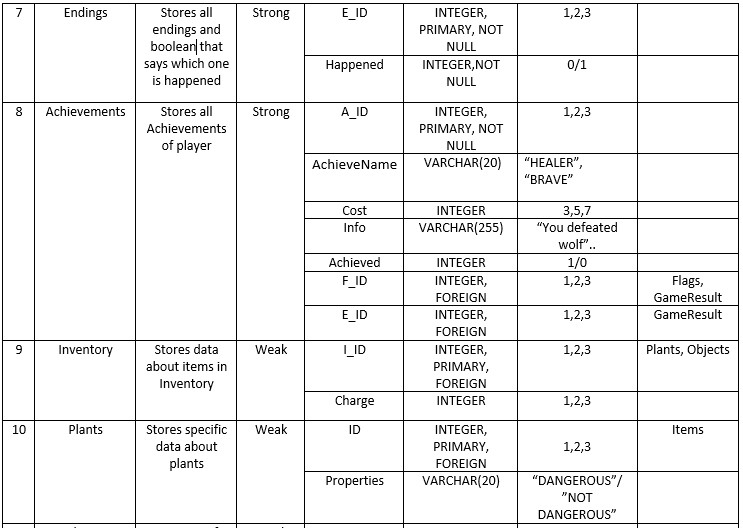
\includegraphics[scale=0.6]{images/LDR3.jpg}
\bigskip
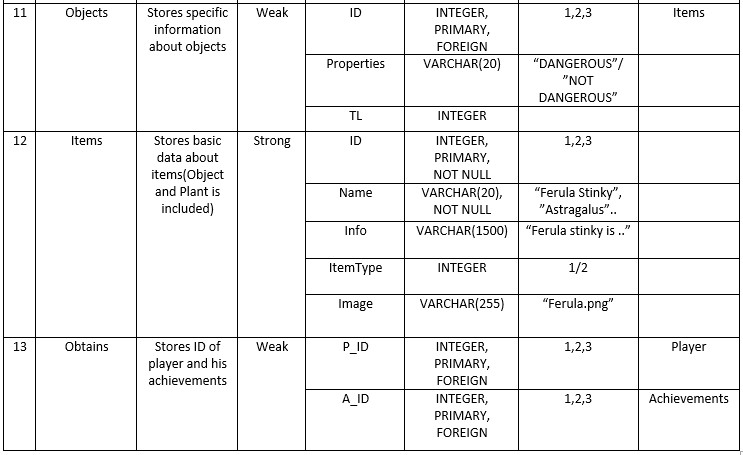
\includegraphics[scale=0.6]{images/LDR4.jpg}
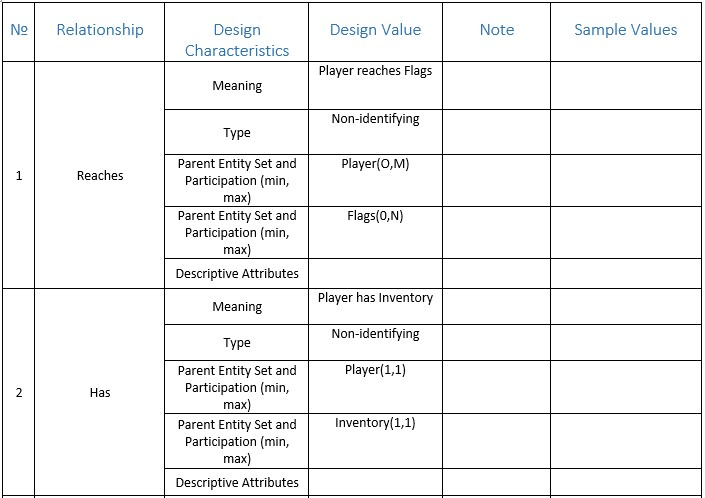
\includegraphics[scale=0.6]{images/LDR5.jpg}
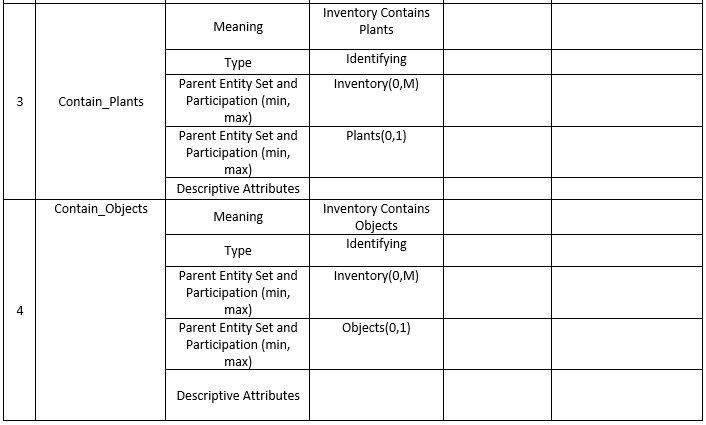
\includegraphics[scale=0.6]{images/LDR6.jpg}
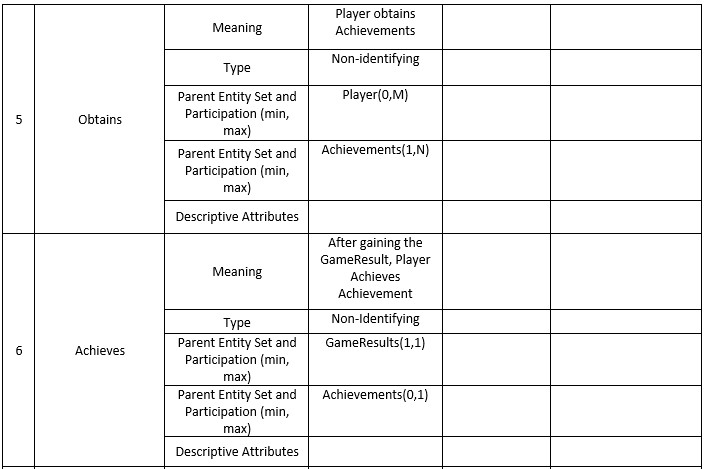
\includegraphics[scale=0.6]{images/LDR7.jpg}     
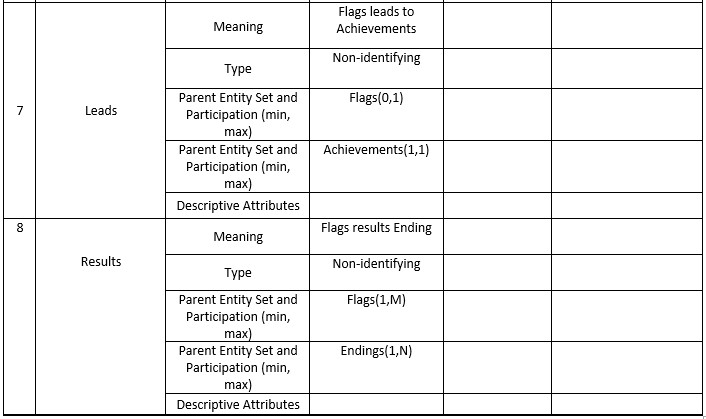
\includegraphics[scale=0.6]{images/LDR8.jpg}
 
\end{center}
\newpage
\subparagraph{3.2 Functional database requirements\\}
\ind\\
1) The system shall have characters with id and name attributes, also characters table should have player and NPC childs.\\
2) The system shall store information about players: score.\\
3) The system shall store information about nonplayable characters: \\
4) The system should know, if the nonplayable character is alive or not, history of the character and the path to his images.\\
5)  The player should have inventory(encyclopedia).\\
6)   There exists items which has plants and objects. Items has info about ID, name, images, item type, info,.\\
7) Plants have their own properties. Plant can heal, hurt, be eaten or do nothing.\\
8) Objects also have their properties. \\
9) In encyclopedia there can be info about plants and objects which player have seen\\
10) Player can reach some flags\\
11) Flags have their own ID, Name and Count. Count is the count of flag, how much does player reached or used this flag.\\
12) After getting needed amount of flag count, player gets to the ending.\\
13) Ending have unique attribute happened. Which indicates does, this ending happened or not.\\
14) System shall store result from flags and endings in flagsum derived attribute \\15) System shall have aggregated table game results where result from flags and endings are stored.\\
\
16) Happening of ending will lead to the game result, which will show what achievements will Player get.\\ 
17) Achievements has attributes, id, name ,achieved, info, and cost. Cost will show the score of the player in the end.\\
18) Also some flags can bring to achievements to. For example: Getting death flag will bring to achievement “Death”\\
19) Player can obtain achievements.\\  
20) Inventory should be weak and depend on plants and objects.\\  

\newpage
\paragraph{4. Design\\}
\subparagraph{4.1 Conceptual database design\\}
\ind\\
Number of Entity Sets: 13\\
Number of Relationship Sets: 8\\
Number of Weak Entity Sets: 8\\
Number of Superclasses/Subclasses: 2/4\\
Number of Aggregate Entity Sets: 1\\
\begin{center}
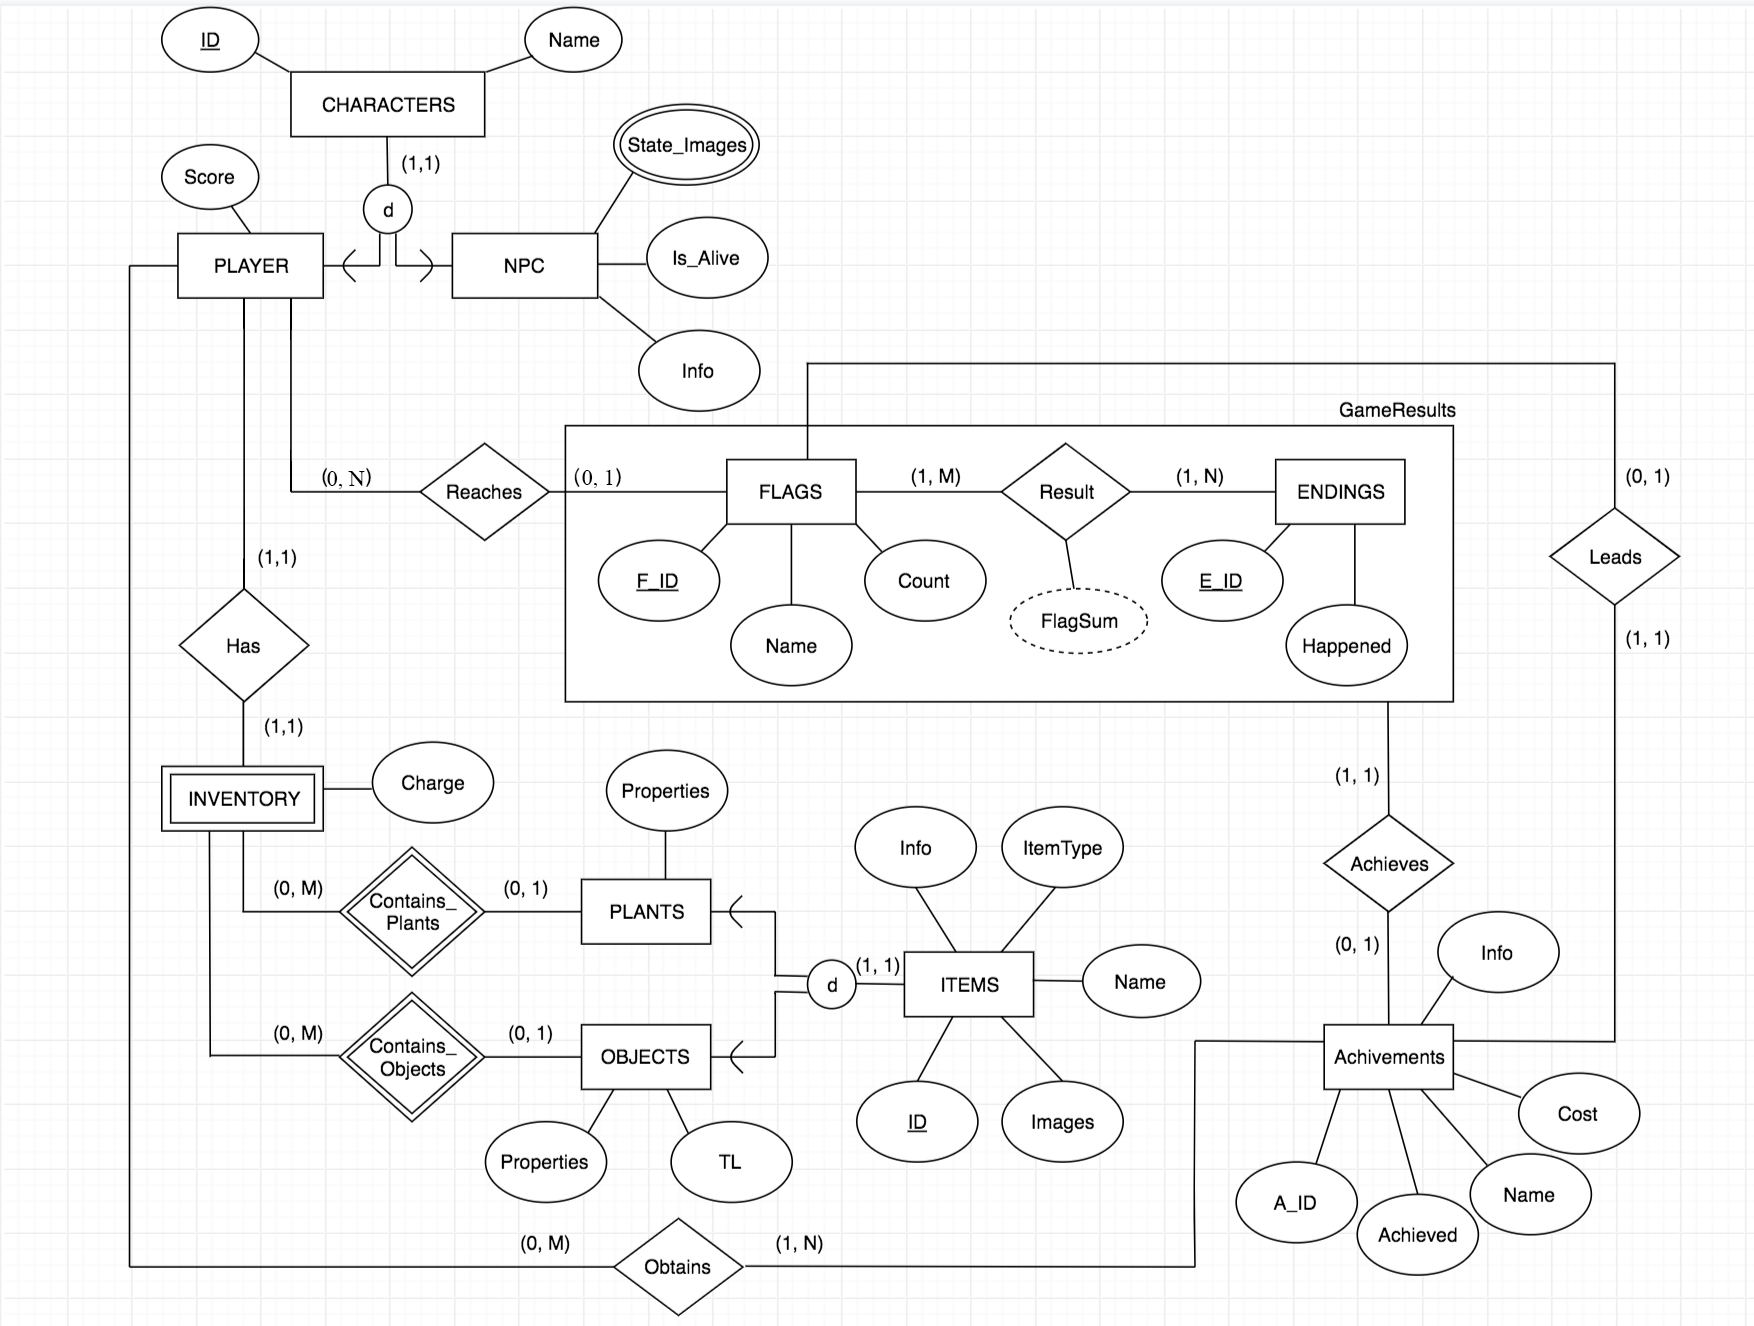
\includegraphics[scale=0.6]{images/Conceptual.png} 
\end{center}
\ind\\
\ind\\
\ind\\
\ind\\
\ind\\
\subparagraph{4.2 Logical database design by ER-Win\\}
\ind\\
Next figures are used to define: Sets/Table - []; Relationships - (); Aggregation - (())\\
\\
\ind 1) Multivalue attribute state\_image in Entity [NPC] in EER has become independent table in ER-Win\\
\ind 2) Relationship (Reaches) has been optimised as foreign key to table [Player] from table [Flags]\\
\ind 3) In EER, [Flags] and [Endigs] Entities have relationship (Result) and their aggregation ((GameResult)) has relationship (Achieved) with Entity [Achivements].In ER-Win, aggregation ((GameResult)) has become independent table and relationship (Result) is optimized into [GameResult] table. \\
\ind 4) Relationship (Leads) has been optimised as foreign key to table [Achievements] from table [Flags]\\
\ind 5) Relationship (Achivies) has been optimised as foreign key to table [Achievements] from aggregation ((GameResult))\\
\ind 6) Relationship (ContainsPlants) which is identifying relationship for [Inventory], has been optimised as foreign key to table [Inventory] from table [Plants]\\
\ind 7)Relationship (ContainObjects) which is identifying relationship for [Inventory], has been optimised as foreign key to table [Inventory] from table [Objects]\\
\begin{center}
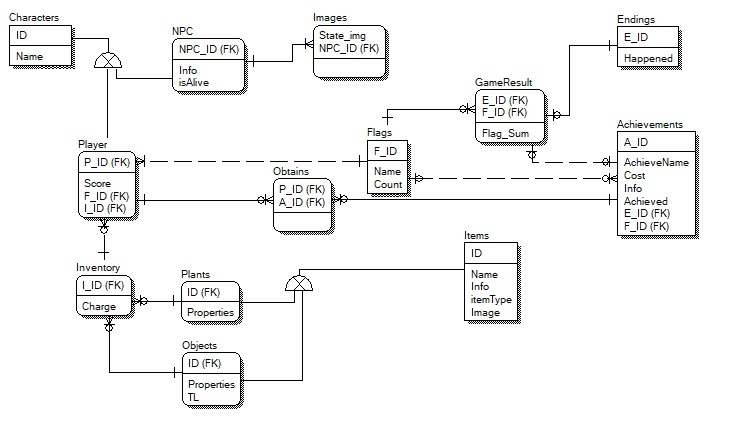
\includegraphics[scale=0.8]{images/Logical.jpg} 
\end{center}
\subparagraph{4.3 Physical database design by ER-Win\\}
\begin{center}
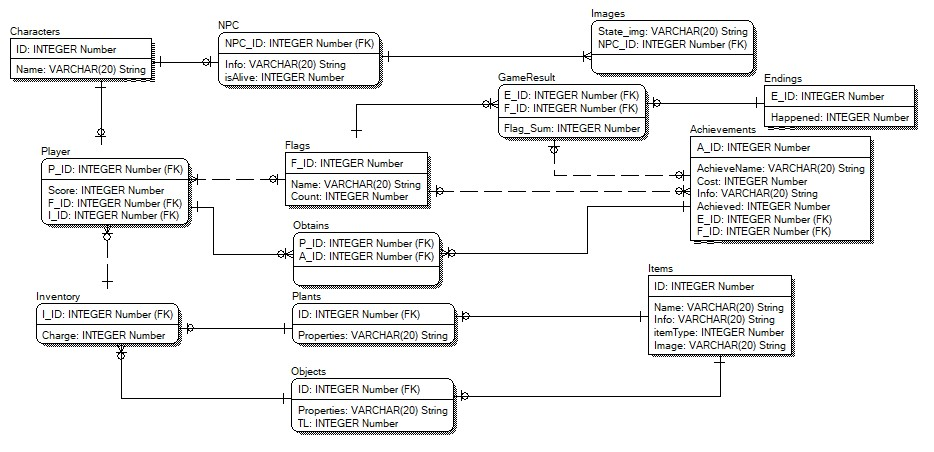
\includegraphics[scale=0.7]{images/Physical.jpg} 
\end{center}
\ind 
\newpage
\paragraph{5. Dependency design\\}

\begin{center}
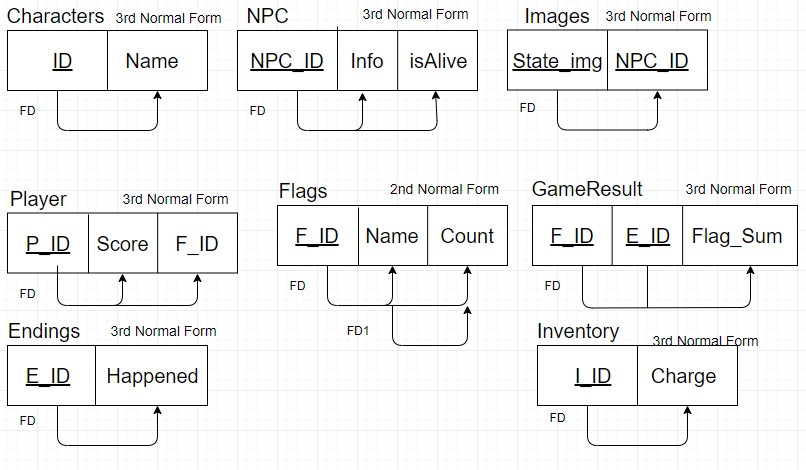
\includegraphics[scale=0.8]{images/FD/FD1.jpg} 
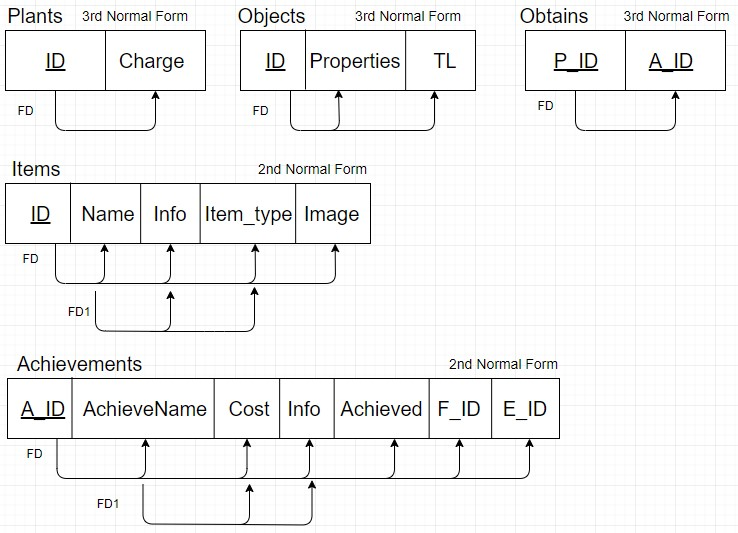
\includegraphics[scale=0.8]{images/FD/FD2.jpg}
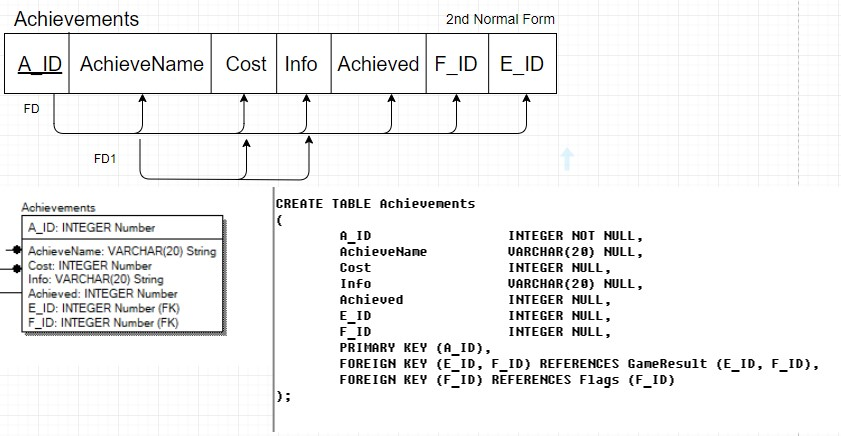
\includegraphics[scale=0.8]{images/FD/FD3.jpg}
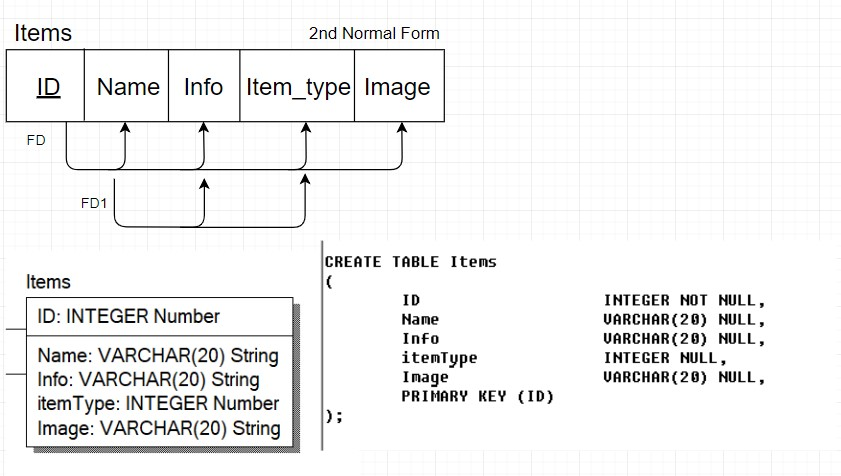
\includegraphics[scale=0.8]{images/FD/FD4.jpg}
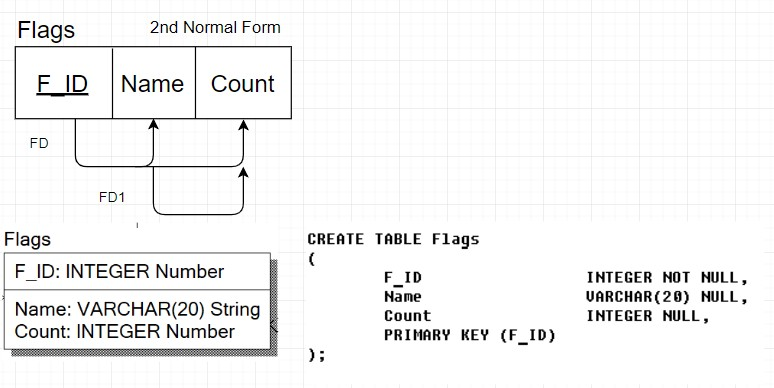
\includegraphics[scale=0.8]{images/FD/FD5.jpg}    
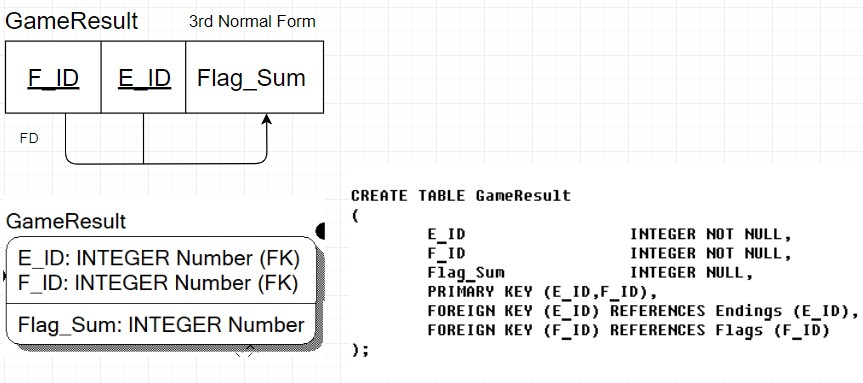
\includegraphics[scale=0.8]{images/FD/FD6.jpg} 
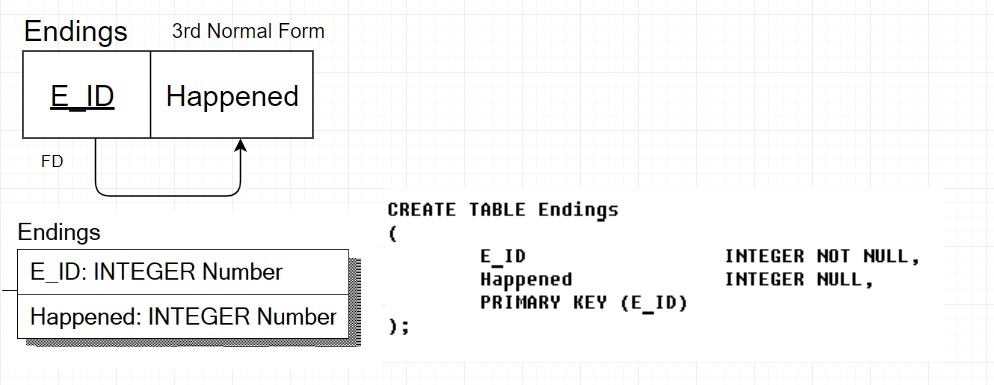
\includegraphics[scale=0.7]{images/FD/FD7.jpg}
\end{center}
\paragraph{6. Interface description\\}
\ind\\
Main Menu contains five buttons: START, OPTIONS, ENCYCLOPEDIA, ACHIEVEMENTS, EXIT.\\
\ind\\START - starts the game itself\\
 OPTIONS - adjust volume of sound\\
ENCYCLOPEDIA - contains information about NPC, plants, animals, items, objects. \textit{Selection} from NPC, Characters and Items table   \\
ACHIEVEMENTS - shows game results like name, cost (how much ''achieved'' costs), info (what you have done), achieved (boolean). \textit{Selection} from Achievements table \\
EXIT - exit/quit game\\
\ind\\
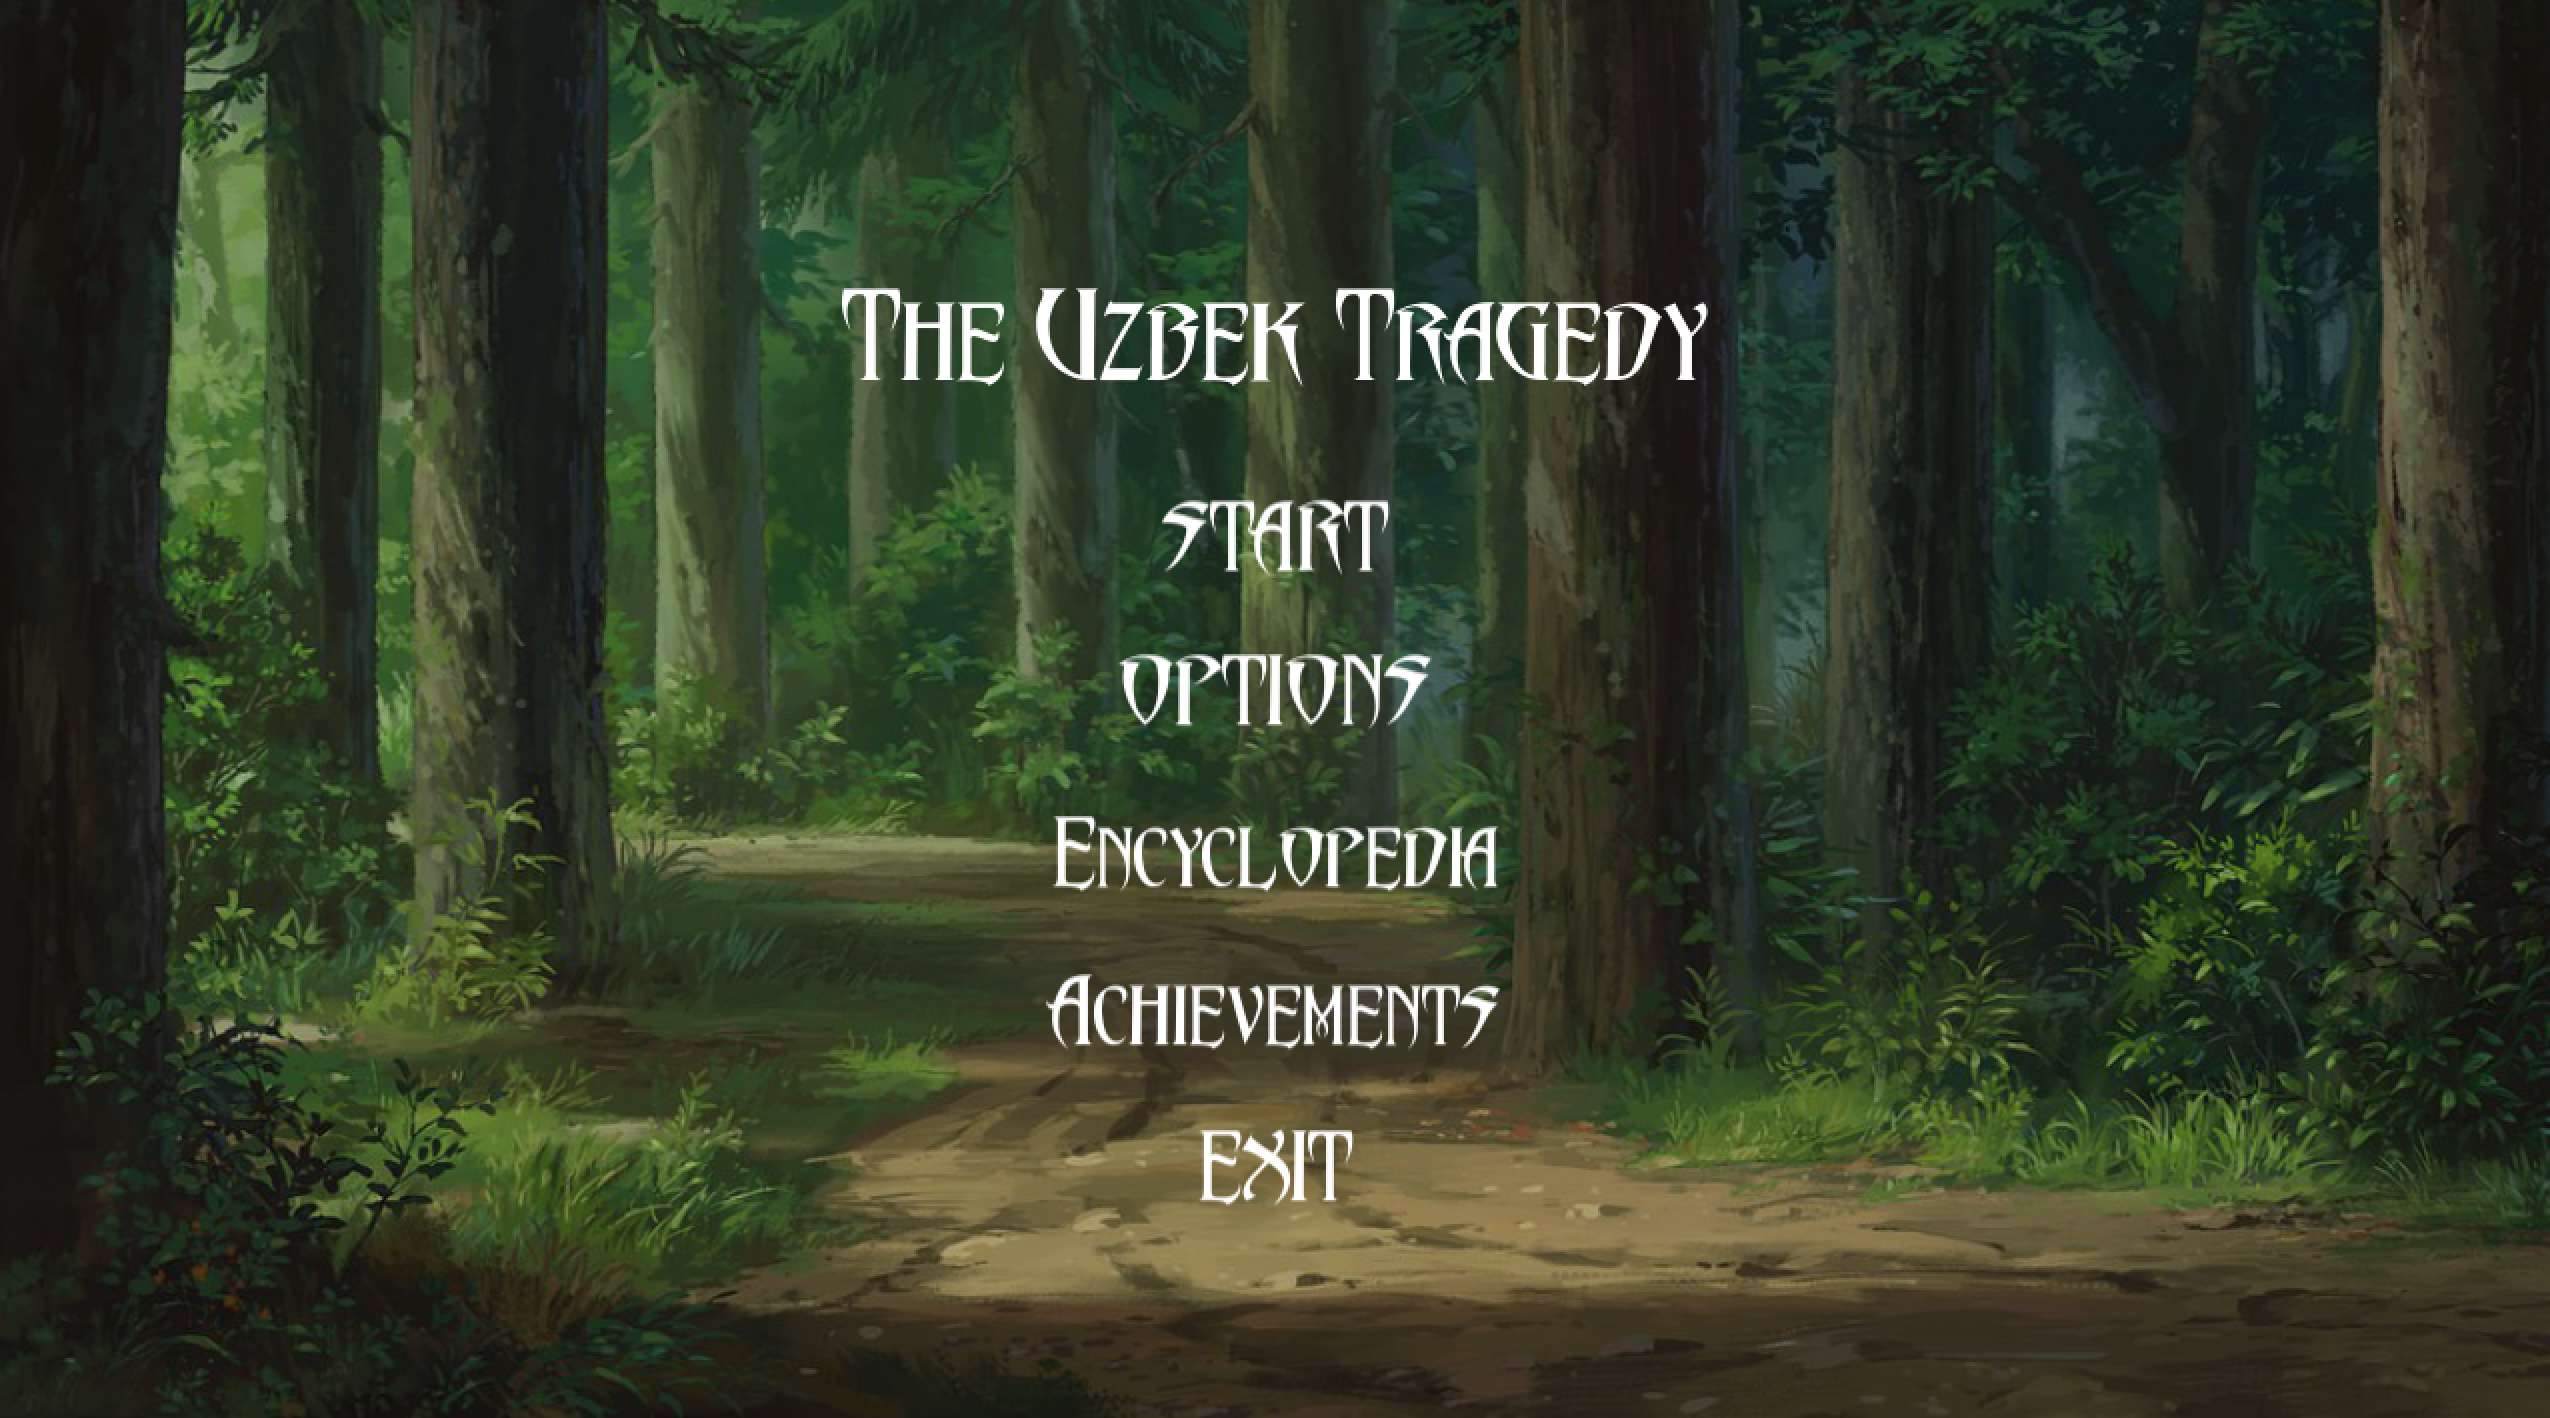
\includegraphics[scale=0.35]{images/menu}
\ind\\ \ind\\
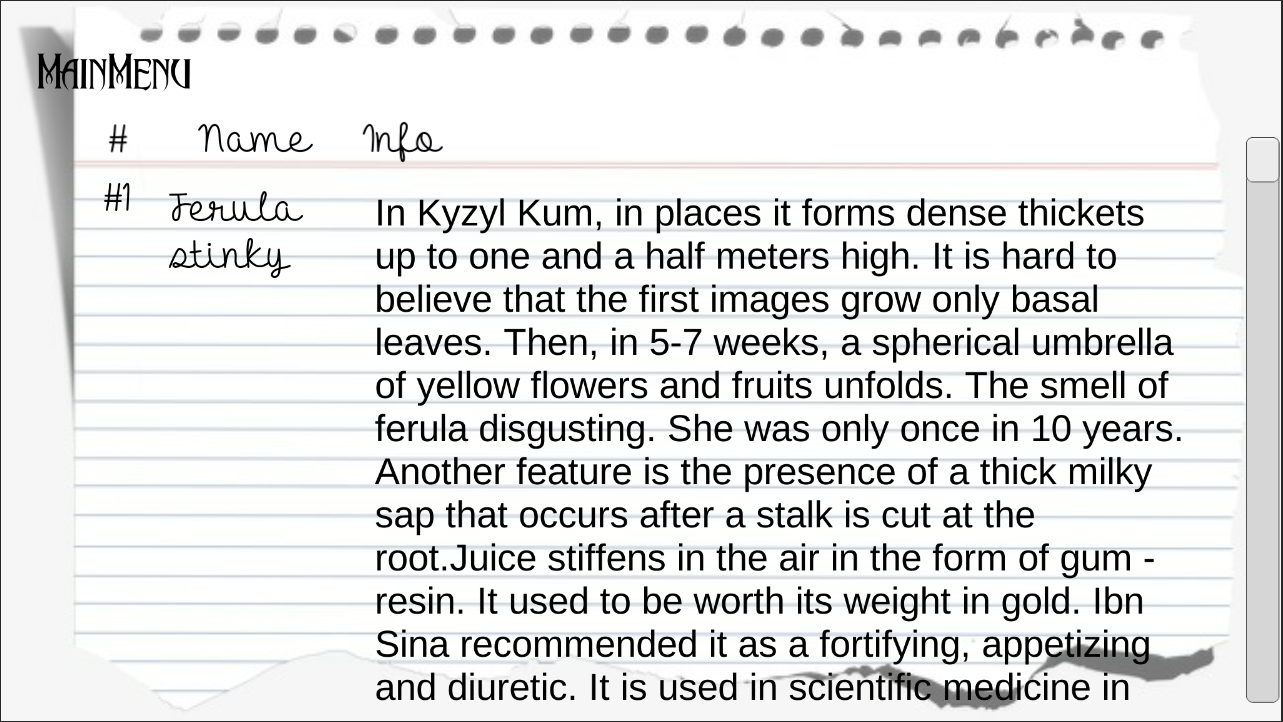
\includegraphics[scale=0.58]{images/en}
\ind\\ \ind\\
As an example, we consider only one story line. After bus accident, a player gets hurt and finds out a plant that can be helpful to heal his wound. The player is supposed to do a choice that change attribute count in the table Flags. Suppose, the player chooses to ''pick a plant''. \textit{Update} of Flags table. Every choice is updating flags table and will lead to any of endings  \\
\ind\\ \ind\\
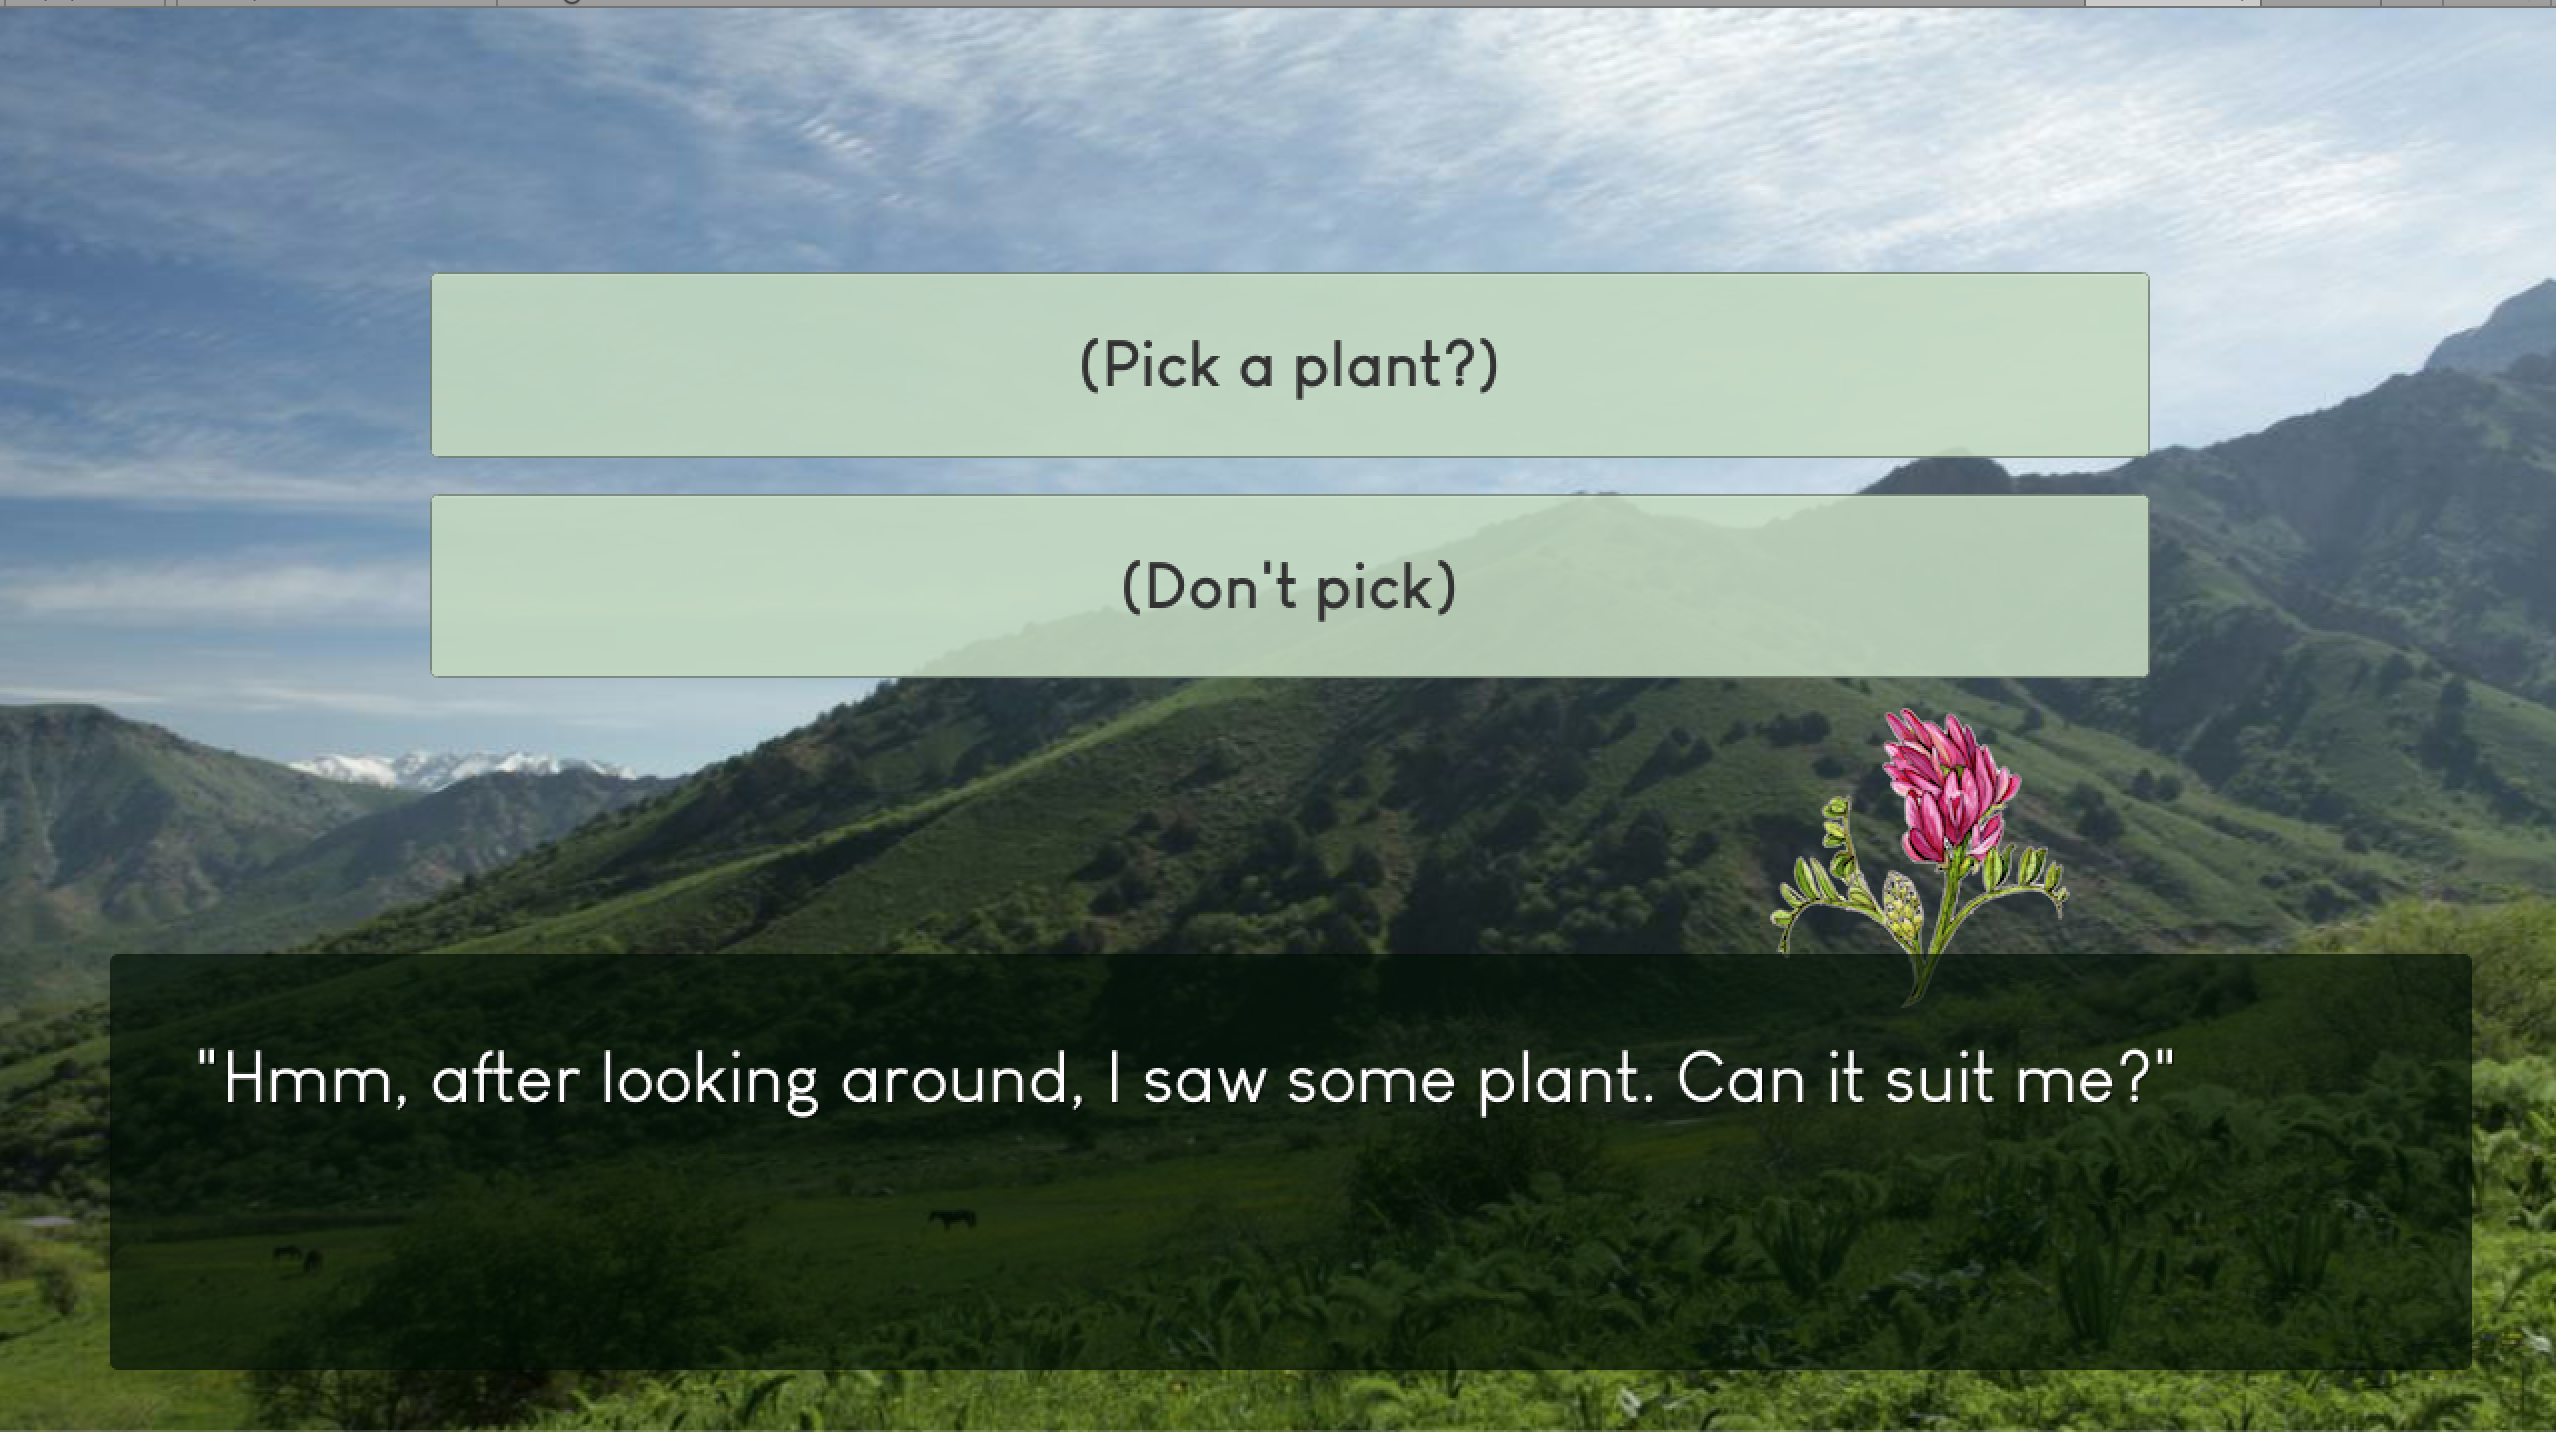
\includegraphics[scale=0.35]{images/1}
\ind\\ \ind\\
After some time, the player again needs to choose, and let it be ''I need to run''. If player would choose I need to fight, he would achieve Brave One Achievement.\\
\\
\ind\\ \ind\\
\includegraphics[scale=0.35]{images/2}
\ind\\ \ind\\
The player is lucky that can avoid the wolf. But it is possible that the player would die, if he initially didn't choose ''pick a plant''. 
\ind\\ \ind\\
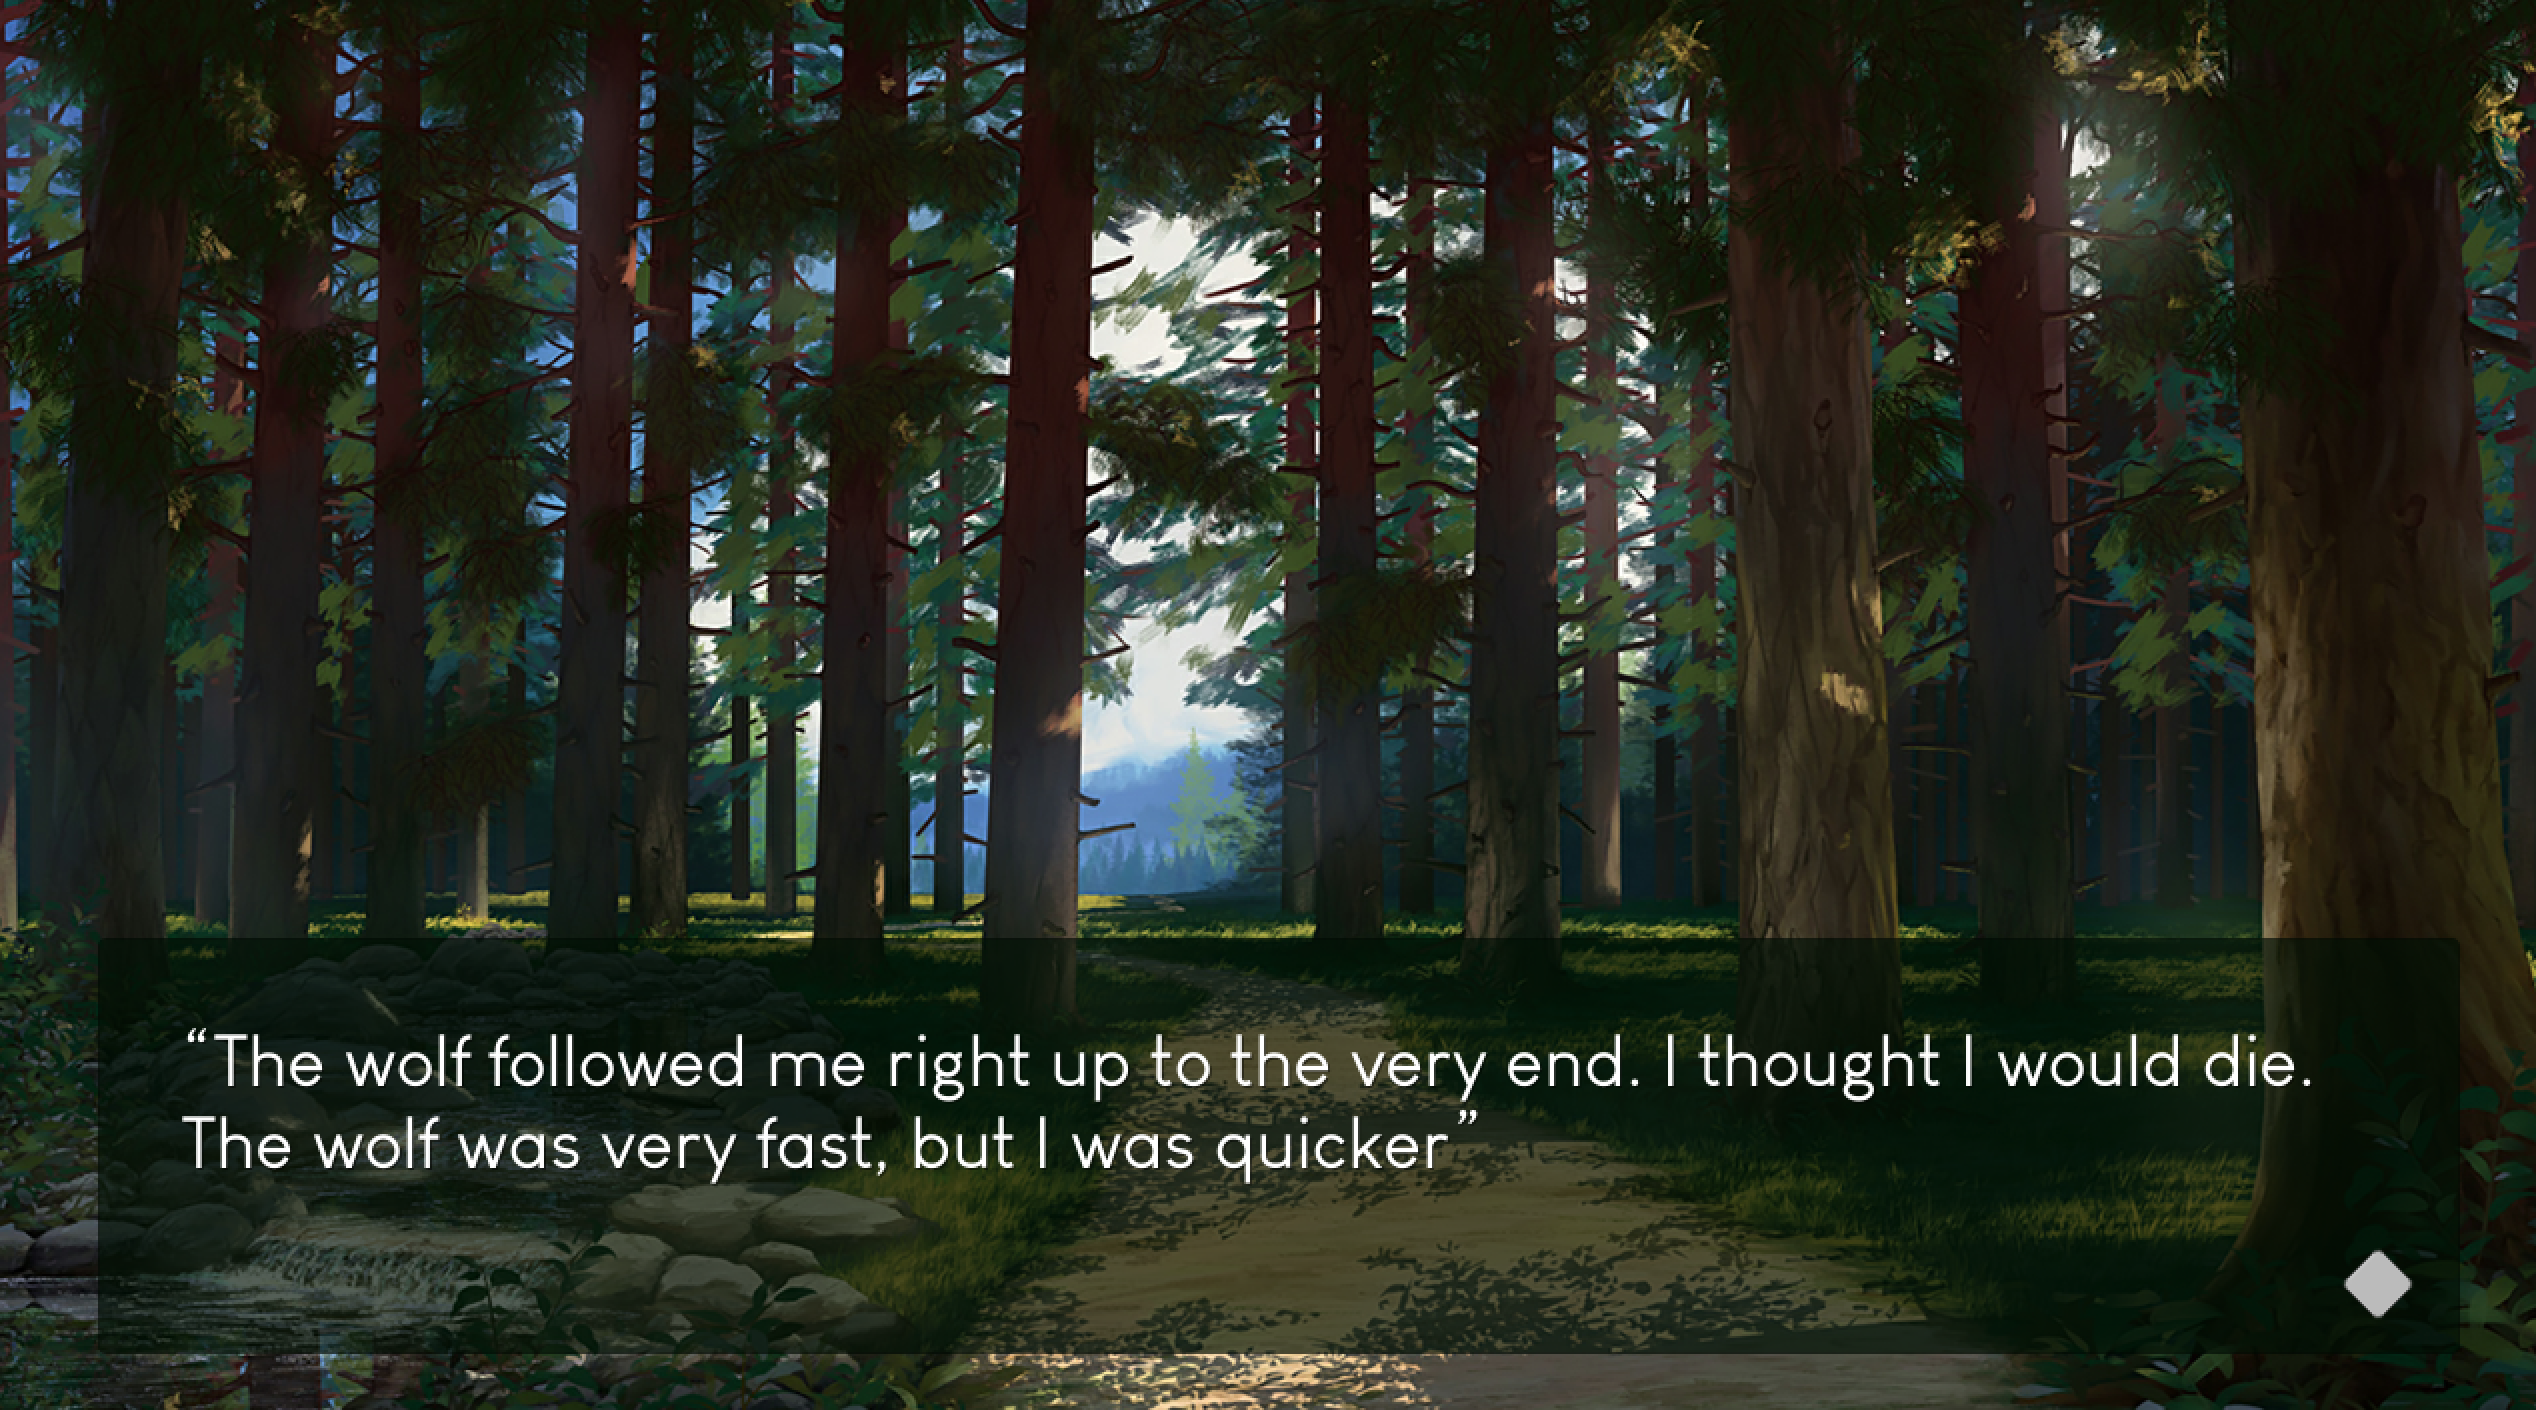
\includegraphics[scale=0.35]{images/3}
\ind\\ \ind\\
And the player encounters with one of his friends (Zod) whom the player's help is needed. Let the player choose ''Help''.\\
\ind\\ \ind\\
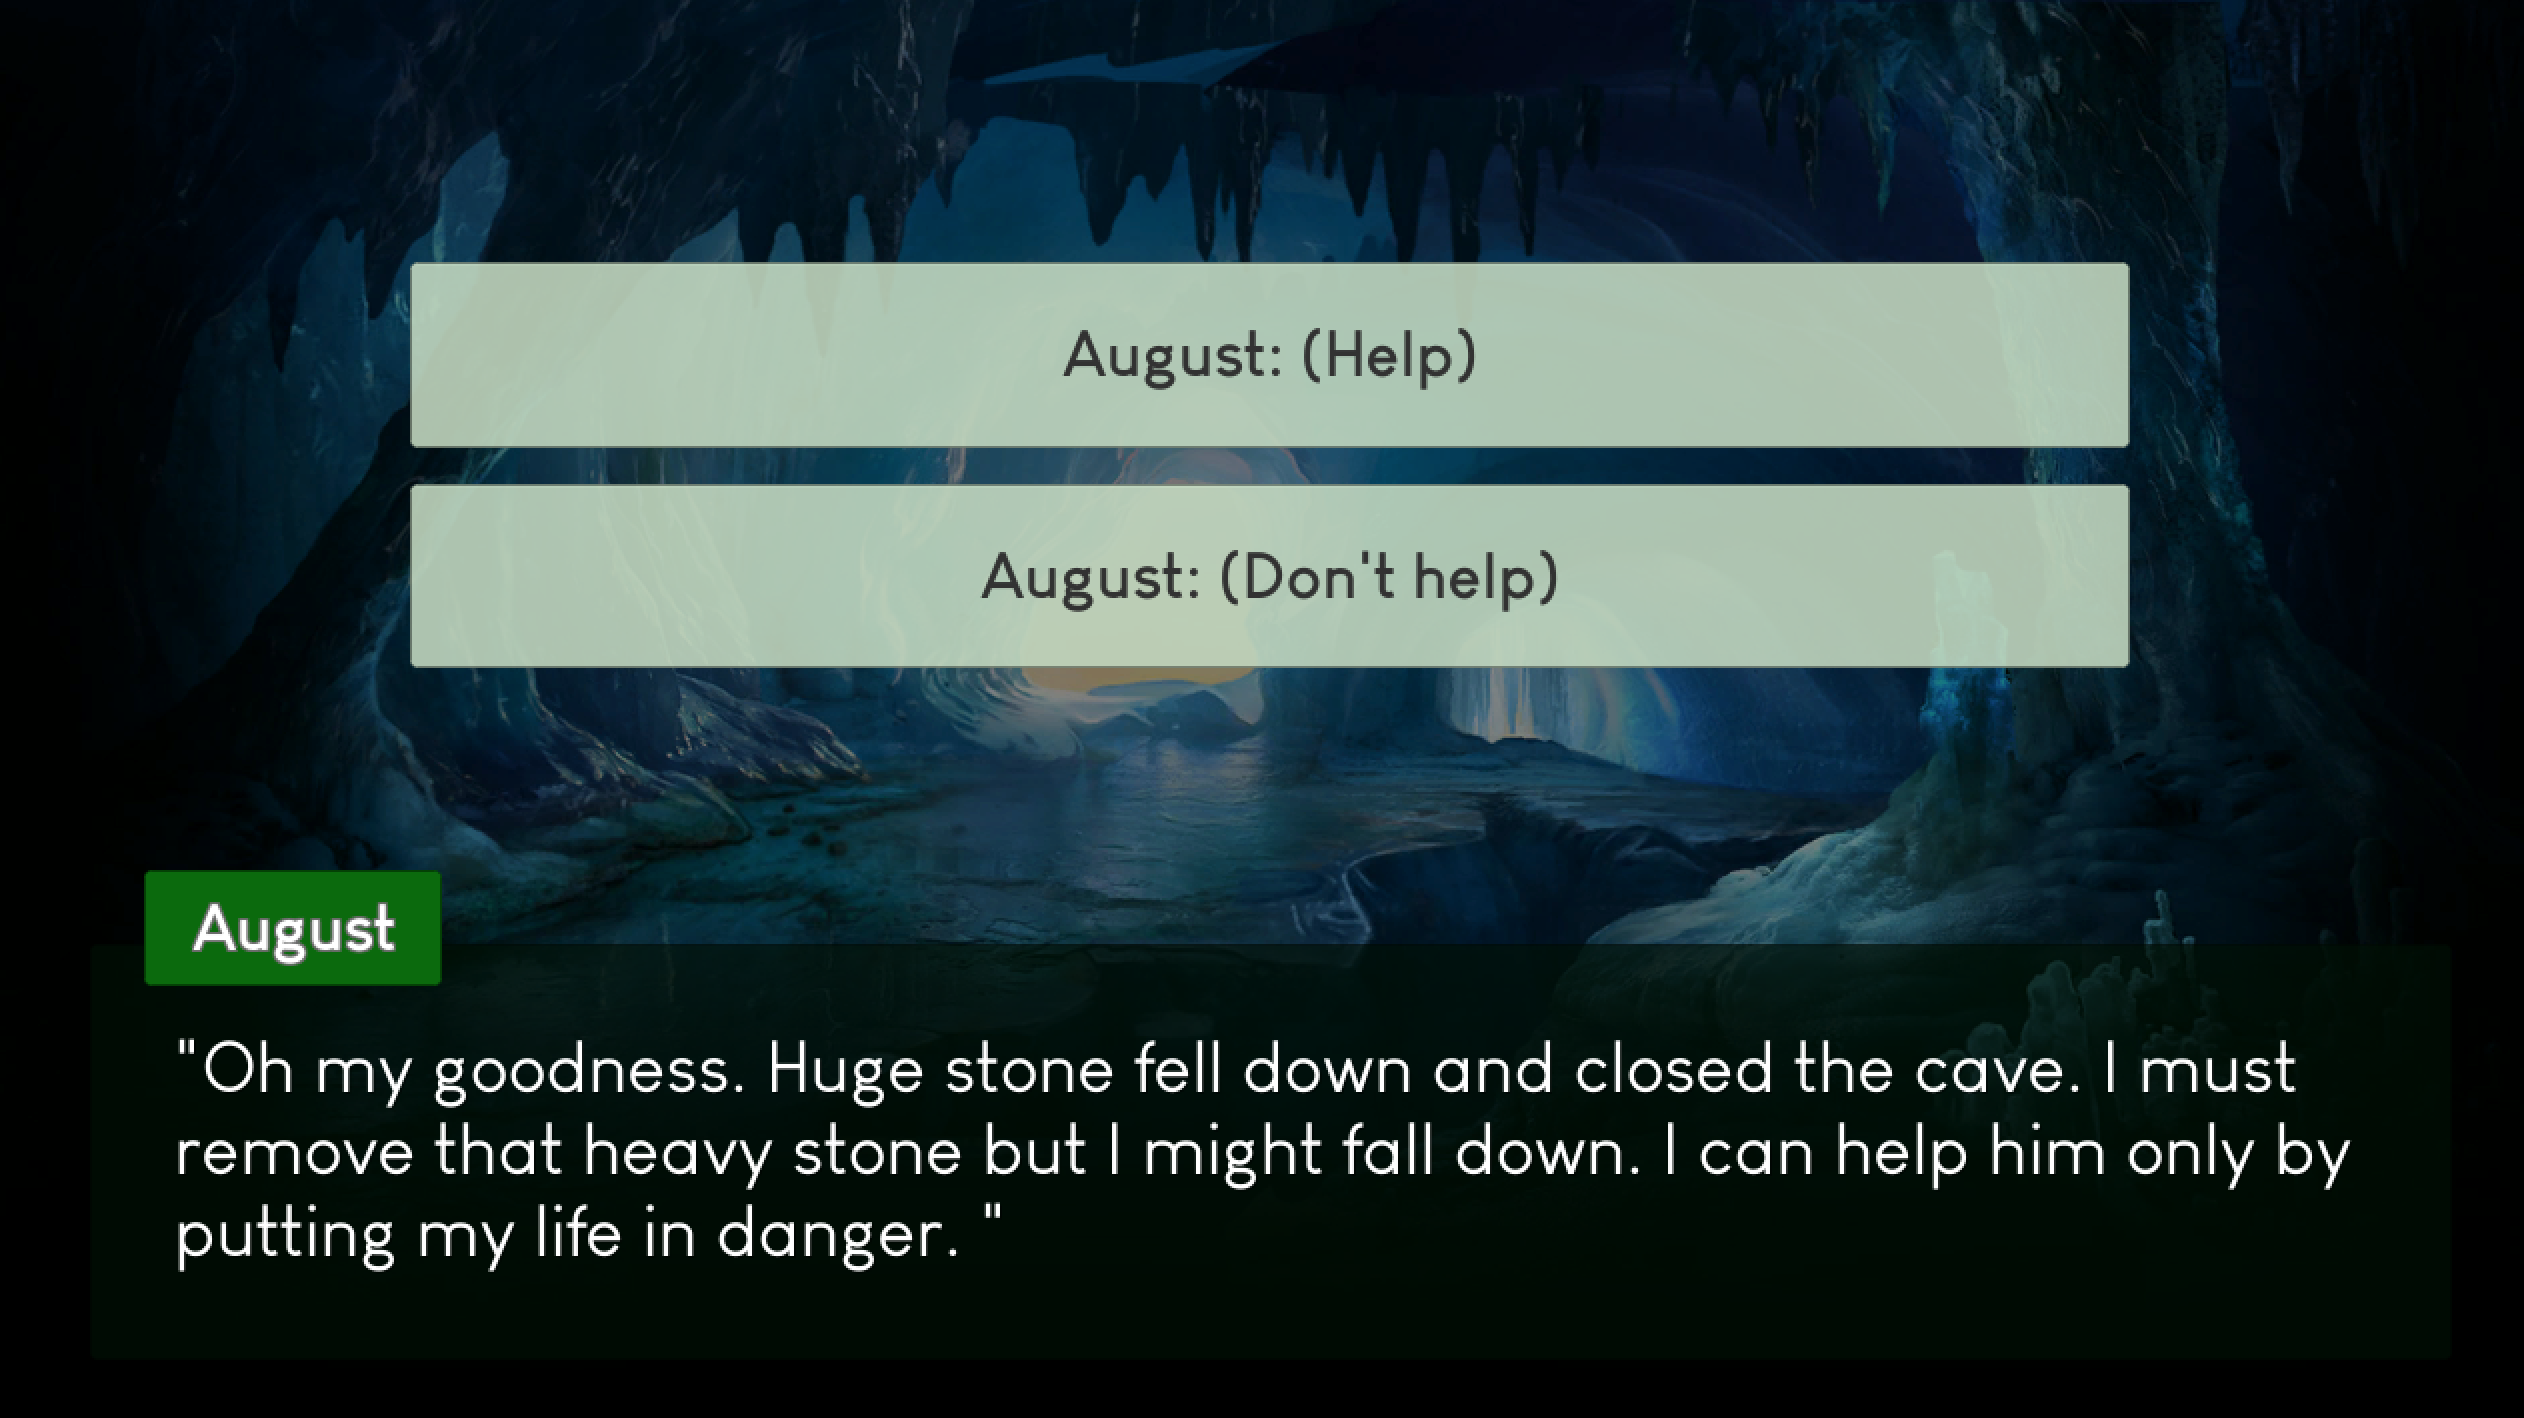
\includegraphics[scale=0.35]{images/4}
\ind\\ \ind\\
Now, the player needs to descent from the mountain with rope or without. 
\ind\\ \ind\\
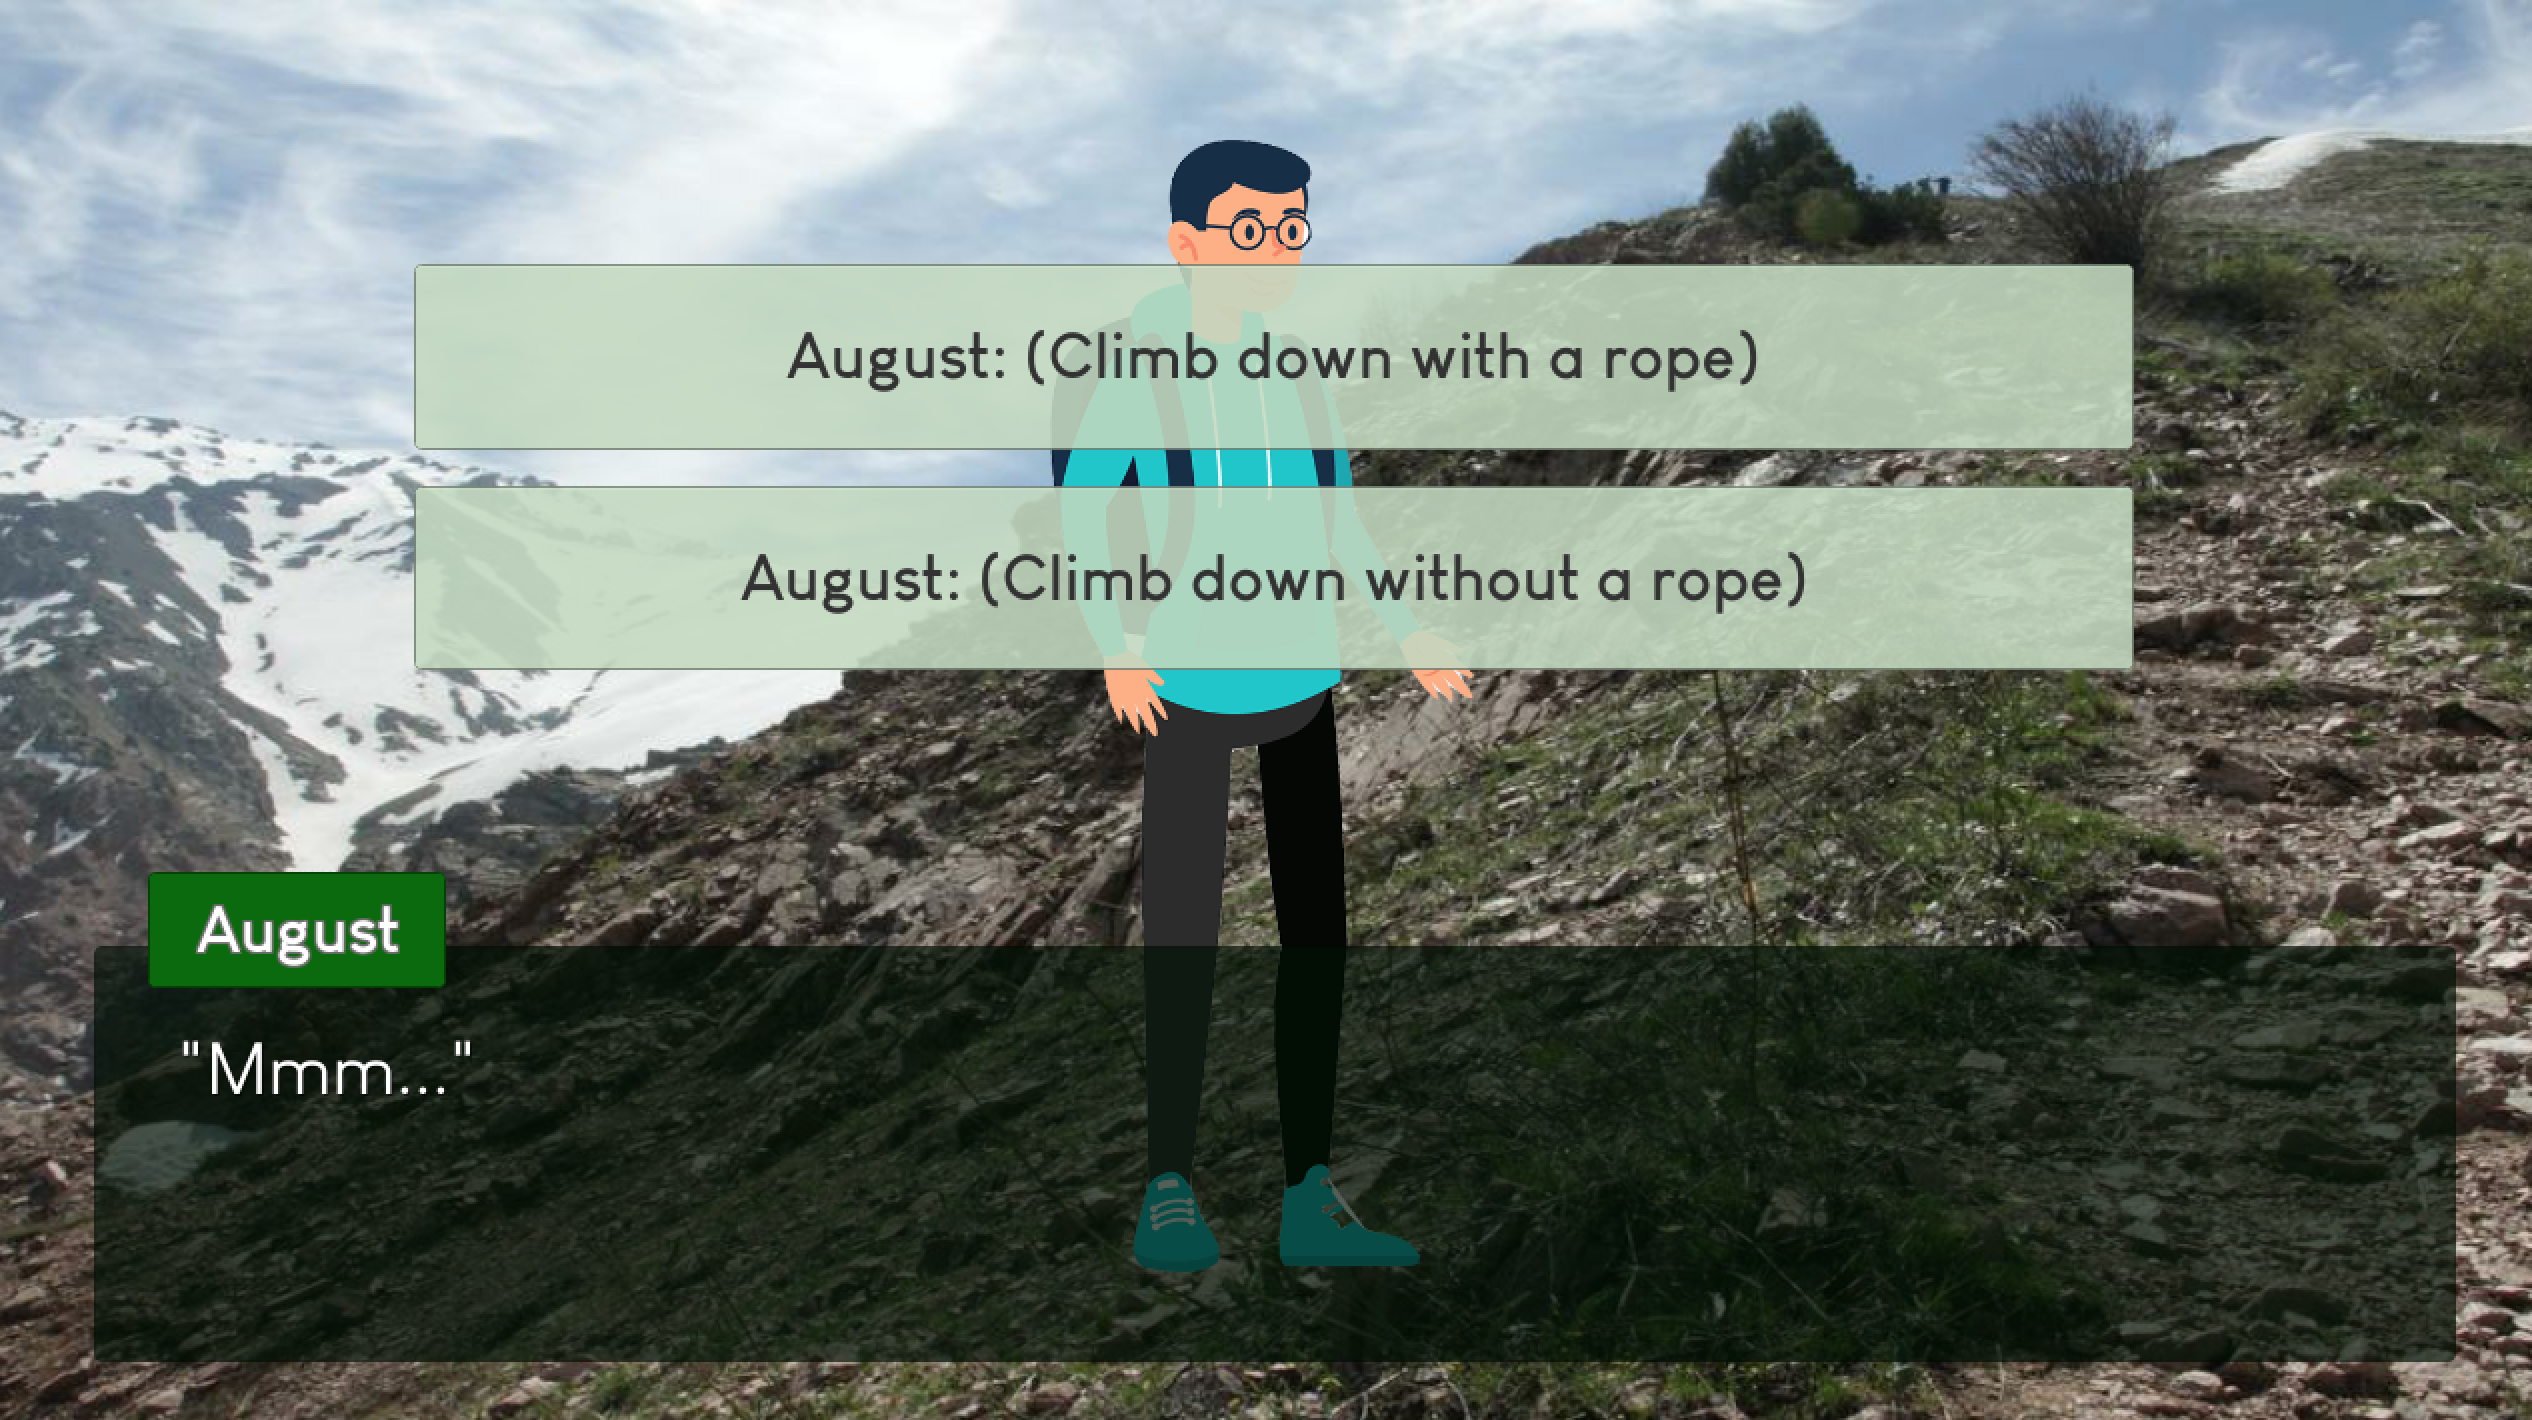
\includegraphics[scale=0.35]{images/5}
\ind\\ \ind\\
The choice ''Climb down with rope'' leads to successful ending. It is the end of game. After the game end, Player will get Game Result \textit{inserting} result into GameResult table, with the Sum of the flags count and ending id showing which ending the player got.\\
\ind\\ \ind\\
\includegraphics[scale=0.35]{images/6}
\ind\\ \ind\\
Here is Achievements of the player illustrating the name, cost, info and achieved attributes.
\ind\\ \ind\\
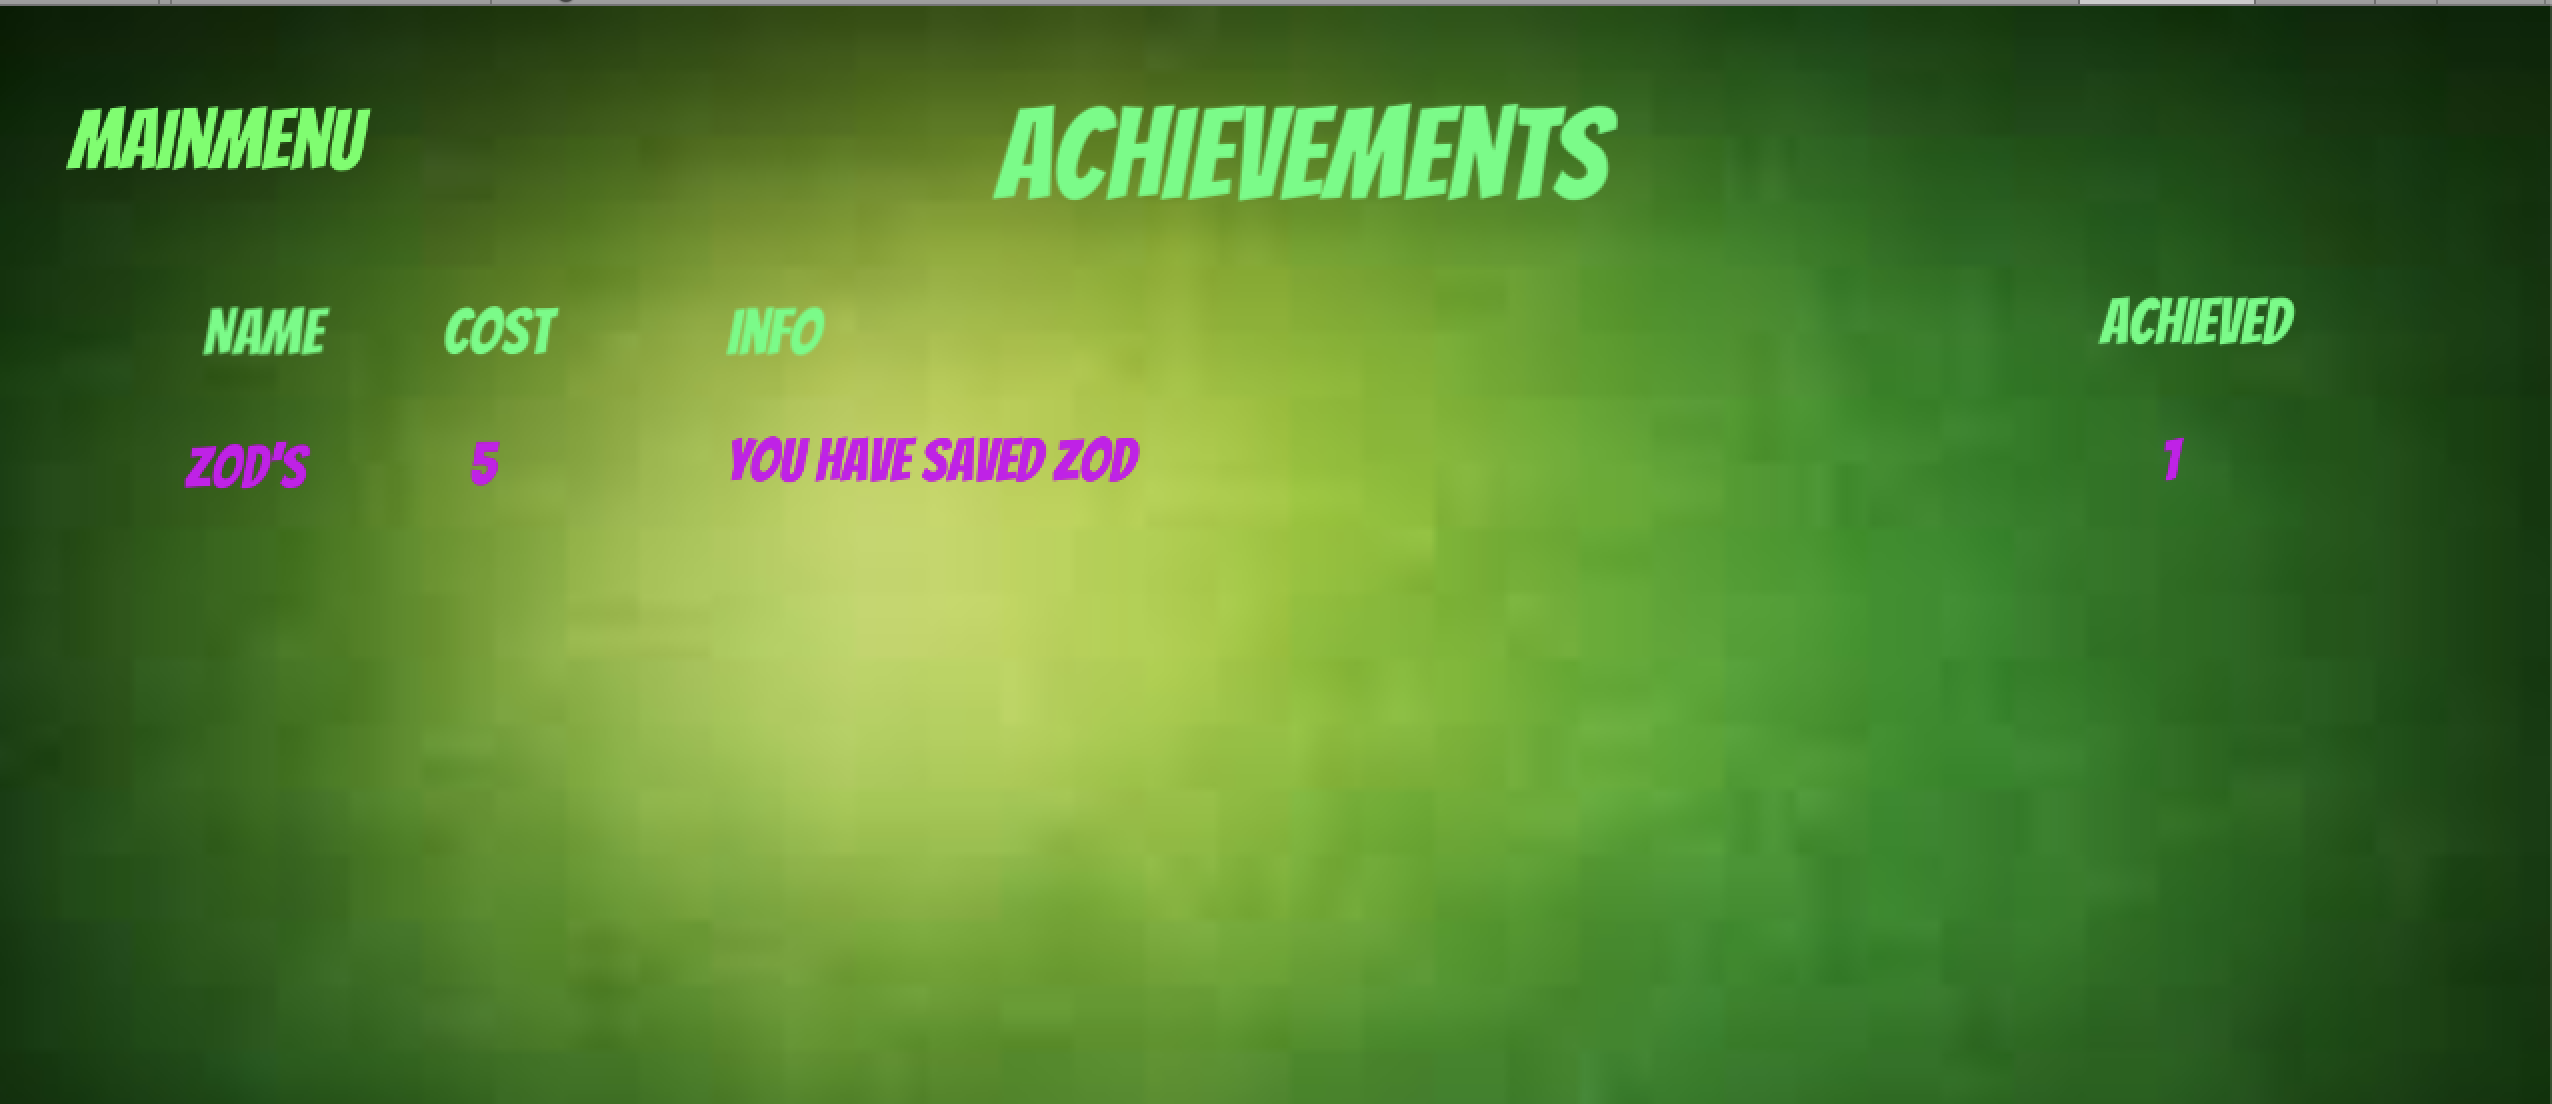
\includegraphics[scale=0.35]{images/achievements}
\ind\\ \ind\\
\paragraph{7. Testing of database\\}
\subparagraph{Plain English\\}
\ind\\
\ind 6. Update players score to 1.\\
\ind 2. Set achieved in Achievements table to 1, meaning that it is true, and player got some achievements.\\
\ind 3. Insert into Obtains table players id and achievements id.\\
\ind 4. Make Gameresult to the sum of flags count. \\
\ind 5. When game is starting set all endings to 0.\\
\ind 6. Characters is a superclass of NPC, so Select everything from characters and npc where chracters id is equal to npc id.\\


\subparagraph{Standard SQL\\}
\ind\\
\ind 1. UPDATE Player SET score = score + 1 WHERE P\_ID = (SELECT P\_ID FROM PLAYER) \\
\ind 2. UPDATE achievements SET achieved = 1, cost = 1 WHERE A\_ID = 1\\
\ind 3. INSERT INTO Obtains values ( (SELECT P\_ID FROM PLAYER) , 1)) \\
\ind 4. INSERT OR REPLACE INTO gameresult VALUES (1, 1, (SELECT SUM(count) as flag\_sum from flags))\\
\ind 5. UPDATE Endings SET Happened = REPLACE(0, E\_ID, 0)\\ 
\ind 6. SELECT * FROM characters INNER JOIN NPC ON id = npc\_id\\


\subparagraph{\textit{DBMS} Screenshots\\}
\ind\\
\ind 1.\\
\begin{center}
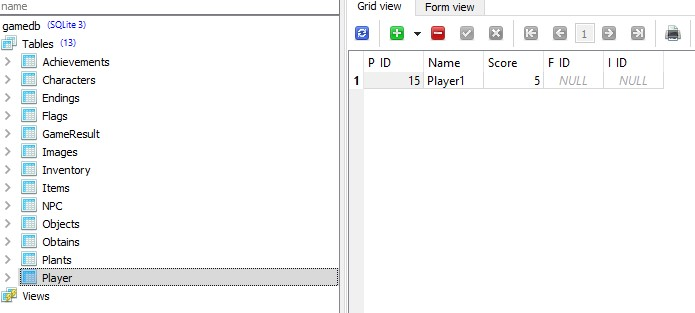
\includegraphics[scale=1]{images/TESTING/DB31.jpg}
\end{center} 
\ind 2.\\
\begin{center}
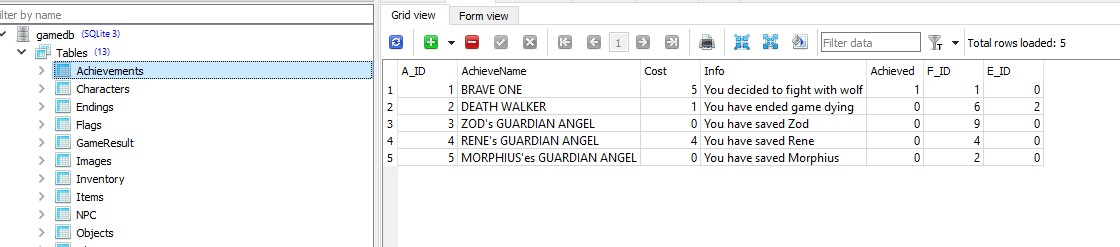
\includegraphics[scale=1]{images/TESTING/DB3.jpg}
\end{center} 
\ind 3.\\
\begin{center}
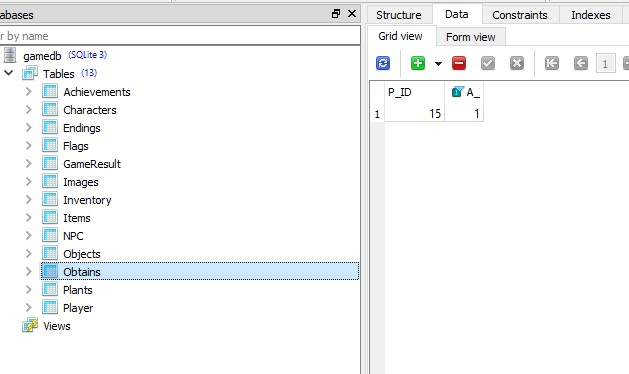
\includegraphics[scale=1]{images/TESTING/DB32.jpg}
\end{center} 
\ind 4.\\
\begin{center}
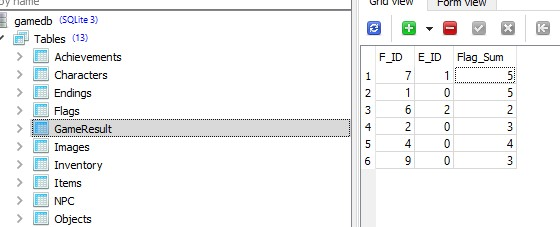
\includegraphics[scale=1]{images/TESTING/DB4.jpg}
\end{center} 
\ind 5.\\
\begin{center}
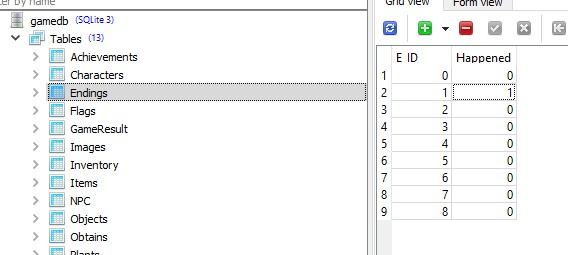
\includegraphics[scale=1]{images/TESTING/DB41.jpg}
\end{center} 
\ind 6.\\
\begin{center}
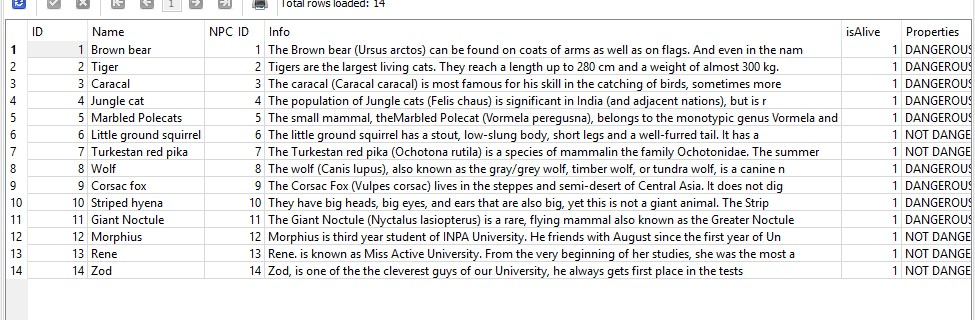
\includegraphics[scale=1]{images/TESTING/DB5.jpg}
\end{center} 
\newpage
\subparagraph{\textit{Interface} Screenshots\\}
\ind\\
\ind 1-3. 
\begin{center}
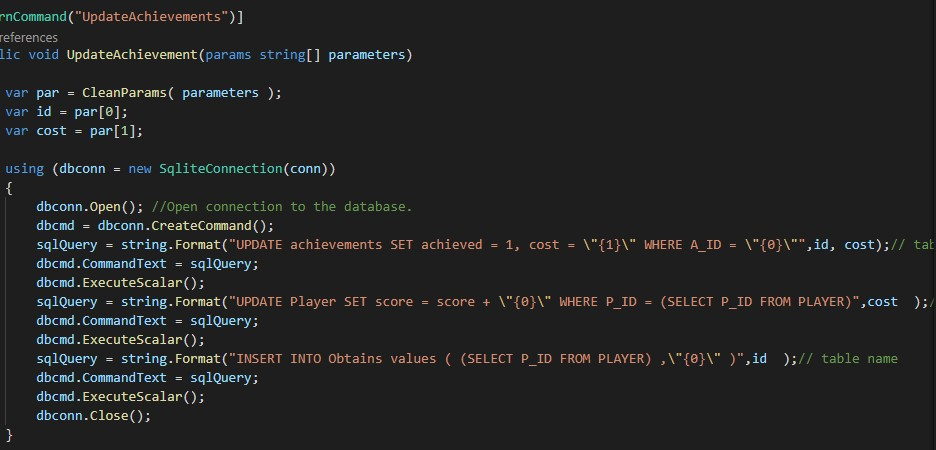
\includegraphics[scale=0.7]{images/TESTING/QUERY3.jpg} \\
\ind\\
\includegraphics[scale=0.385]{images/TESTING/2.png} \\
\end{center}
\newpage
\ind\indent 4-5.\\
\begin{center}
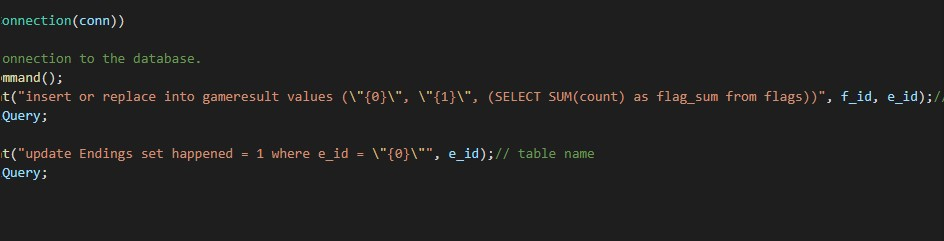
\includegraphics[scale=0.7]{images/TESTING/QUERY4.jpg} \\
\ind\\
\includegraphics[scale=0.385]{images/TESTING/6.png} \\
\end{center}
\newpage
\ind\indent 6.\\
\begin{center}
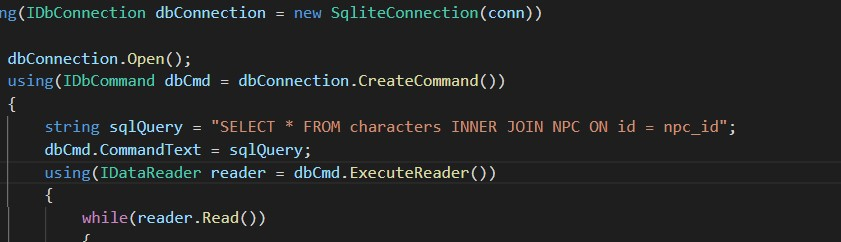
\includegraphics[scale=0.8]{images/TESTING/QUERY5.jpg} \\
\ind\\
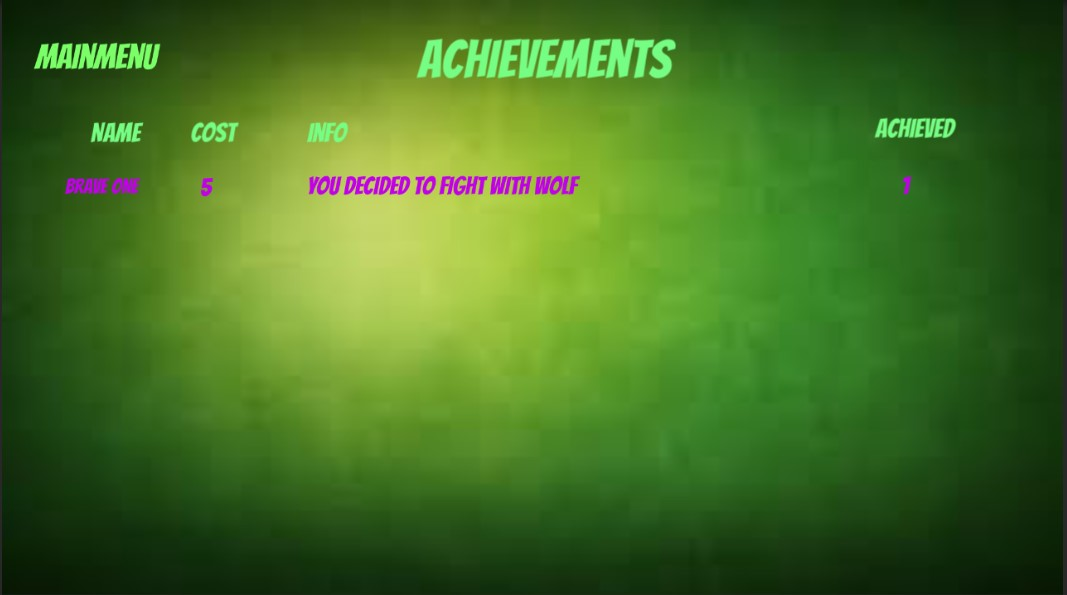
\includegraphics[scale=0.6]{images/TESTING/Achievements.jpg} 
\end{center}
\ind\\
\ind\\
\ind\\ In this SQL queries 1 means number taken from the system.
\newpage
\begin{thebibliography}{9}
\bibitem{unity} 
Unity platform,
\\\texttt{https://unity.com/}
\bibitem{fate} 
Fate Stay night,
\\\texttt{http://www.typemoon.com/products/fate/index.html}
\bibitem{shoujo} 
Katawa shoujo,
\\\texttt{https://www.katawa-shoujo.com/}
\bibitem{summer} 
Everlasting Summer
\\\texttt{http://www.typemoon.com/products/fate/index.html}
\end{thebibliography}

\end{document}

